
\documentclass[xcolor=dvipsnames]{beamer}  % for hardcopy add 'trans'

\mode<presentation>
{
  \usetheme{Singapore}
  % or ...
  \setbeamercovered{transparent}
  % or whatever (possibly just delete it)
}

\usefonttheme{professionalfonts}
\usepackage[russian]{babel}
% or whatever
%\usepackage[latin1]{inputenc}
% or whatever
%\usepackage{times}
%\usepackage[T1]{fontenc}
% Or whatever. Note that the encoding and the font should match. If T1
% does not look nice, try deleting the line with the fontenc.

%%%%%%%%%%%%%%%%%%%%%% start my preamble %%%%%%%%%%%%%%%%%%%%%%


\addtobeamertemplate{navigation symbols}{}{%
    \usebeamerfont{footline}%
    \usebeamercolor[fg]{footline}%
    \hspace{1em}%
    \insertframenumber/\inserttotalframenumber
} 

\setbeamercolor{footline}{fg=blue}
\setbeamerfont{footline}{series=\bfseries}


%\usepackage{epsfig}
\usepackage{graphicx}
\graphicspath{{./figs_code/}}

\usepackage{amsmath, amssymb, amsthm}

\usepackage{fancyvrb}

\usepackage{tikz}
\usetikzlibrary{arrows}
\usetikzlibrary{calc}
\usetikzlibrary{intersections}
\usetikzlibrary{decorations}
\usepackage{pgf}
\usepackage{pgfplots}
\pgfplotsset{compat=1.13}

\usepackage{graphviz}
 
\usepackage{verbatim}


\usepackage{algorithmicx,algpseudocode}


%font
\usepackage{mathpazo}
%\usepackage[usenames, dvipsnames]{color}

%\usepackage[linesnumbered, ruled, lined]{algorithm2e}

\usepackage{xr}
\externaldocument[ET-]{et}


\newcommand*{\theorembreak}{\usebeamertemplate{theorem end}\framebreak\usebeamertemplate{theorem begin}}

\newcommand{\newtopic}[1]{\textcolor{Green}{\Large \bf #1}}
\newcommand{\navy}[1]{\textcolor{Blue}{\bf #1}}
\newcommand{\navymth}[1]{\textcolor{Blue}{#1}}
\newcommand{\red}[1]{\textcolor{red}{#1}}


\definecolor{pale}{RGB}{235, 235, 235}
\definecolor{pale2}{RGB}{175,238,238}
\definecolor{turquois4}{RGB}{0,134,139}

% Typesetting code
\definecolor{bg}{rgb}{0.95,0.95,0.95}
\usepackage{minted}
\usemintedstyle{friendly}
\newminted{python}{mathescape,frame=lines,framesep=4mm,bgcolor=bg}
\newminted{ipython}{mathescape,frame=lines,framesep=4mm,bgcolor=bg}
\newminted{julia}{mathescape,frame=lines,framesep=4mm,bgcolor=bg}
\newminted{c}{mathescape,linenos=true}
\newminted{r}{mathescape,  frame=none, baselinestretch=1, framesep=2mm}
\renewcommand{\theFancyVerbLine}{\sffamily
    \textcolor[rgb]{0.5,0.5,1.0}{\scriptsize {\arabic{FancyVerbLine}}}}


\usepackage{stmaryrd}

\newcommand{\Fact}{\textcolor{Brown}{\bf Факт. }}
\newcommand{\Facts}{\textcolor{Brown}{\bf Факты }}
\newcommand{\keya}{\textcolor{turquois4}{\bf Ключевая идея. }}
\newcommand{\Factnodot}{\textcolor{Brown}{\bf Факт }}
\newcommand{\Eg}{\textcolor{ForestGreen}{Пример. }}
\newcommand{\Egs}{\textcolor{ForestGreen}{Примеры. }}
\newcommand{\Ex}{{\bf Ex. }}
\newcommand{\Thm}{\textcolor{Brown}{\bf Теорема. }}
\newcommand{\Prf}{\textcolor{turquois4}{\bf Доказательство. }}
\newcommand{\Ass}{\textcolor{turquois4}{\bf Допущение.}} 
\newcommand{\Lem}{\textcolor{Brown}{\bf Лемма. }}

%source code 



% cali
\usepackage{mathrsfs}
\usepackage{bbm}
\usepackage{subfigure}

\newcommand{\argmax}{\operatornamewithlimits{argmax}}
\newcommand{\argmin}{\operatornamewithlimits{argmin}}

\newcommand\T{{\mathpalette\raiseT\intercal}}
\newcommand\raiseT[2]{\raisebox{0.25ex}{$#1#2$}}

\DeclareMathOperator{\cl}{cl}
%\DeclareMathOperator{\argmax}{argmax}
\DeclareMathOperator{\interior}{int}
\DeclareMathOperator{\Prob}{Prob}
\DeclareMathOperator{\kernel}{ker}
\DeclareMathOperator{\diag}{diag}
\DeclareMathOperator{\sgn}{sgn}
\DeclareMathOperator{\determinant}{det}
\DeclareMathOperator{\trace}{trace}
\DeclareMathOperator{\Span}{span}
\DeclareMathOperator{\rank}{rank}
\DeclareMathOperator{\cov}{cov}
\DeclareMathOperator{\corr}{corr}
\DeclareMathOperator{\range}{rng}
\DeclareMathOperator{\var}{var}
\DeclareMathOperator{\mse}{mse}
\DeclareMathOperator{\se}{se}
\DeclareMathOperator{\row}{row}
\DeclareMathOperator{\col}{col}
\DeclareMathOperator{\dimension}{dim}
\DeclareMathOperator{\fracpart}{frac}
\DeclareMathOperator{\proj}{proj}
\DeclareMathOperator{\colspace}{colspace}

\providecommand{\inner}[1]{\left\langle{#1}\right\rangle}

% mics short cuts and symbols
% mics short cuts and symbols
\newcommand{\st}{\ensuremath{\ \mathrm{s.t.}\ }}
\newcommand{\setntn}[2]{ \{ #1 : #2 \} }
\newcommand{\cf}[1]{ \lstinline|#1| }
\newcommand{\otms}[1]{ \leftidx{^\circ}{#1}}

\newcommand{\fore}{\therefore \quad}
\newcommand{\tod}{\stackrel { d } {\to} }
\newcommand{\tow}{\stackrel { w } {\to} }
\newcommand{\toprob}{\stackrel { p } {\to} }
\newcommand{\toms}{\stackrel { ms } {\to} }
\newcommand{\eqdist}{\stackrel {\textrm{ \scriptsize{d} }} {=} }
\newcommand{\iidsim}{\stackrel {\textrm{ {\sc iid }}} {\sim} }
\newcommand{\1}{\mathbbm 1}
\newcommand{\dee}{\,{\rm d}}
\newcommand{\given}{\, | \,}
\newcommand{\la}{\langle}
\newcommand{\ra}{\rangle}

\renewcommand{\rho}{\varrho}

\newcommand{\htau}{ \hat \tau }
\newcommand{\hgamma}{ \hat \gamma }

\newcommand{\boldx}{ {\mathbf x} }
\newcommand{\boldu}{ {\mathbf u} }
\newcommand{\boldv}{ {\mathbf v} }
\newcommand{\boldw}{ {\mathbf w} }
\newcommand{\boldy}{ {\mathbf y} }
\newcommand{\boldb}{ {\mathbf b} }
\newcommand{\bolda}{ {\mathbf a} }
\newcommand{\boldc}{ {\mathbf c} }
\newcommand{\boldi}{ {\mathbf i} }
\newcommand{\bolde}{ {\mathbf e} }
\newcommand{\boldp}{ {\mathbf p} }
\newcommand{\boldq}{ {\mathbf q} }
\newcommand{\bolds}{ {\mathbf s} }
\newcommand{\boldt}{ {\mathbf t} }
\newcommand{\boldz}{ {\mathbf z} }

\newcommand{\boldzero}{ {\mathbf 0} }
\newcommand{\boldone}{ {\mathbf 1} }

\newcommand{\boldalpha}{ {\boldsymbol \alpha} }
\newcommand{\boldbeta}{ {\boldsymbol \beta} }
\newcommand{\boldgamma}{ {\boldsymbol \gamma} }
\newcommand{\boldtheta}{ {\boldsymbol \theta} }
\newcommand{\boldxi}{ {\boldsymbol \xi} }
\newcommand{\boldtau}{ {\boldsymbol \tau} }
\newcommand{\boldepsilon}{ {\boldsymbol \epsilon} }
\newcommand{\boldmu}{ {\boldsymbol \mu} }
\newcommand{\boldSigma}{ {\boldsymbol \Sigma} }
\newcommand{\boldOmega}{ {\boldsymbol \Omega} }
\newcommand{\boldPhi}{ {\boldsymbol \Phi} }
\newcommand{\boldLambda}{ {\boldsymbol \Lambda} }
\newcommand{\boldphi}{ {\boldsymbol \phi} }

\newcommand{\Sigmax}{ {\boldsymbol \Sigma_{\boldx}}}
\newcommand{\Sigmau}{ {\boldsymbol \Sigma_{\boldu}}}
\newcommand{\Sigmaxinv}{ {\boldsymbol \Sigma_{\boldx}^{-1}}}
\newcommand{\Sigmav}{ {\boldsymbol \Sigma_{\boldv \boldv}}}

\newcommand{\hboldx}{ \hat {\mathbf x} }
\newcommand{\hboldy}{ \hat {\mathbf y} }
\newcommand{\hboldb}{ \hat {\mathbf b} }
\newcommand{\hboldu}{ \hat {\mathbf u} }
\newcommand{\hboldtheta}{ \hat {\boldsymbol \theta} }
\newcommand{\hboldtau}{ \hat {\boldsymbol \tau} }
\newcommand{\hboldmu}{ \hat {\boldsymbol \mu} }
\newcommand{\hboldbeta}{ \hat {\boldsymbol \beta} }
\newcommand{\hboldgamma}{ \hat {\boldsymbol \gamma} }
\newcommand{\hboldSigma}{ \hat {\boldsymbol \Sigma} }

\newcommand{\boldA}{\mathbf A}
\newcommand{\boldB}{\mathbf B}
\newcommand{\boldC}{\mathbf C}
\newcommand{\boldD}{\mathbf D}
\newcommand{\boldI}{\mathbf I}
\newcommand{\boldL}{\mathbf L}
\newcommand{\boldM}{\mathbf M}
\newcommand{\boldP}{\mathbf P}
\newcommand{\boldQ}{\mathbf Q}
\newcommand{\boldR}{\mathbf R}
\newcommand{\boldX}{\mathbf X}
\newcommand{\boldU}{\mathbf U}
\newcommand{\boldV}{\mathbf V}
\newcommand{\boldW}{\mathbf W}
\newcommand{\boldY}{\mathbf Y}
\newcommand{\boldZ}{\mathbf Z}

\newcommand{\bSigmaX}{ {\boldsymbol \Sigma_{\hboldbeta}} }
\newcommand{\hbSigmaX}{ \mathbf{\hat \Sigma_{\hboldbeta}} }

\newcommand{\RR}{\mathbbm R}
\newcommand{\CC}{\mathbbm C}
\newcommand{\NN}{\mathbbm N}
\newcommand{\PP}{\mathbbm P}
\newcommand{\EE}{\mathbbm E \nobreak\hspace{.1em}}
\newcommand{\EEP}{\mathbbm E_P \nobreak\hspace{.1em}}
\newcommand{\ZZ}{\mathbbm Z}
\newcommand{\QQ}{\mathbbm Q}


\newcommand{\XX}{\mathcal X}

\newcommand{\aA}{\mathcal A}
\newcommand{\fF}{\mathscr F}
\newcommand{\bB}{\mathscr B}
\newcommand{\iI}{\mathscr I}
\newcommand{\rR}{\mathscr R}
\newcommand{\dD}{\mathcal D}
\newcommand{\lL}{\mathcal L}
\newcommand{\llL}{\mathcal{H}_{\ell}}
\newcommand{\gG}{\mathcal G}
\newcommand{\hH}{\mathcal H}
\newcommand{\nN}{\textrm{\sc n}}
\newcommand{\lN}{\textrm{\sc ln}}
\newcommand{\pP}{\mathscr P}
\newcommand{\qQ}{\mathscr Q}
\newcommand{\xX}{\mathcal X}

\newcommand{\ddD}{\mathscr D}


\newcommand{\R}{{\texttt R}}
\newcommand{\risk}{\mathcal R}
\newcommand{\Remp}{R_{{\rm emp}}}

\newcommand*\diff{\mathop{}\!\mathrm{d}}
\newcommand{\ess}{ \textrm{{\sc ess}} }
\newcommand{\tss}{ \textrm{{\sc tss}} }
\newcommand{\rss}{ \textrm{{\sc rss}} }
\newcommand{\rssr}{ \textrm{{\sc rssr}} }
\newcommand{\ussr}{ \textrm{{\sc ussr}} }
\newcommand{\zdata}{\mathbf{z}_{\mathcal D}}
\newcommand{\Pdata}{P_{\mathcal D}}
\newcommand{\Pdatatheta}{P^{\mathcal D}_{\theta}}
\newcommand{\Zdata}{Z_{\mathcal D}}


\newcommand{\e}[1]{\mathbbm{E}[{#1}]}
\newcommand{\p}[1]{\mathbbm{P}({#1})}

%\theoremstyle{plain}
%\newtheorem{axiom}{Axiom}[section]
%\newtheorem{theorem}{Theorem}[section]
%\newtheorem{corollary}{Corollary}[section]
%\newtheorem{lemma}{Lemma}[section]
%\newtheorem{proposition}{Proposition}[section]
%
%\theoremstyle{definition}
%\newtheorem{definition}{Definition}[section]
%\newtheorem{example}{Example}[section]
%\newtheorem{remark}{Remark}[section]
%\newtheorem{notation}{Notation}[section]
%\newtheorem{assumption}{Assumption}[section]
%\newtheorem{condition}{Condition}[section]
%\newtheorem{exercise}{Ex.}[section]
%\newtheorem{fact}{Fact}[section]

% Bibliography
\usepackage[authordate,uniquename=false,firstinits,backend=biber,maxcitenames=2]{biblatex-chicago}
\DeclareFieldFormat[article]{title}{#1}
\DeclareFieldFormat[inproceedings]{title}{#1}
\addbibresource{et_newbib.bib}
\renewcommand{\cite}{\textcite}



\setlength{\parskip}{1.5ex plus0.5ex minus0.5ex}


\setlength{\jot}{12pt} 










\title{Учебник по Эконометрике}

\subtitle
{Лекция 2: Линейная Алгебра и Матрицы}

\author{Джон Стачурски \\ \vspace{0.5em} 
	\scriptsize Лекции: Акшай Шенкер \\ \vspace{0.1em} 
	\scriptsize Перевел: Алексей Кедо}




\begin{document}

\begin{frame}
  \titlepage
\end{frame}

\section{Матрицы и Линейные уравнения}

\begin{frame}
    
    \vspace{2em}
    \frametitle{Матрицы}

    Обычная \navy{$N \times K$ матрица}: 
    
    \begin{equation*}
        \boldA = 
        \left(
        \begin{array}{cccc}
            a_{11} & a_{12} & \cdots & a_{1K} \\
            a_{21} & a_{22} & \cdots & a_{2K} \\
            \vdots & \vdots &  & \vdots \\
            a_{N1} & a_{N2} & \cdots & a_{NK} 
        \end{array}
        \right)
    \end{equation*}
    %
    
    \vspace{.7em}
    Символ $a_{nk}$ означает элемент, стоящий в $n$-ой строке $k$-ого столбца

\end{frame}


\begin{frame}
    
    \vspace{2em}
    $N \times K$ матрица также называется 
    %
    \begin{itemize}
        \item \navy{вектором строки}, если $N = 1$
        \item \navy{вектором столбца}, если $K = 1$
    \end{itemize}
    
    \vspace{.7em}
    Если $N = K$, то матрицу $\boldA$ называют \navy{квадратной}
    
    Если $\boldA$ квадратная и $a_{nk} = a_{kn}$ для любых $k$ и $n$, то $\boldA$
    называют \navy{симметричной}   
    
\end{frame}

\begin{frame}

    \vspace{2em}
    Часто элементы матрицы $\boldA$ представляют собой коэффициенты 
    в системе линейных уравнений
    %
    \begin{equation*}
        \label{eq:sleq}
        \begin{array}{c}
            a_{11} x_1 + a_{12} x_2 + \cdots + a_{1K} x_K = b_1 \\
            \vdots  \\
            a_{N1} x_1 + a_{N2} x_2 + \cdots + a_{NK} x_K = b_N 
        \end{array}
    \end{equation*}
    
\end{frame}

\begin{frame}

    \vspace{2em}
    Для матрицы $\boldA$ применяются обозначения:
    \begin{itemize}
        \item $\row_n \boldA$ означает
    $n$-ую строку $\boldA$
        \item $\col_k \boldA$ означает $k$-ый столбец $\boldA$
    \end{itemize} 
    
    \vspace{.7em}
    Символы $\boldzero$ и $\boldone$ представляют собой матрицы, 
    все элементы которых равны нулю и единице соответственно
    
\end{frame}

\begin{frame}
    
    \vspace{2em}
    Для квадратной матрицы $\boldA$, элементы $a_{nn}$ называют \navy{главной диагональю}:
    %
    \begin{equation*}
        \left(
        \begin{array}{cccc}
            \red{a_{11}} & a_{12} & \cdots & a_{1N} \\
            a_{21} & \red{a_{22}} & \cdots & a_{2N} \\
            \vdots & \vdots &  & \vdots \\
            a_{N1} & a_{N2} & \cdots & \red{a_{NN}} \\
        \end{array}
        \right)
    \end{equation*}
    %

    \navy{Единичная матрица}:
    %
    \begin{equation*}
        \boldI := 
        \left(
        \begin{array}{cccc}
            1 & 0 & \cdots & 0 \\
            0 & 1 & \cdots & 0 \\
            \vdots & \vdots &  & \vdots \\
            0 & 0 & \cdots & 1 \\
        \end{array}
        \right)
    \end{equation*}
    %
    Заметим, что $\col_n \boldI = \bolde_n$ --- $n$-ый канонический базис $\RR^N$
    

\end{frame}

\begin{frame}
    \frametitle{Алгебраические операции над матрицами}

    \vspace{2em}
    Операции над матрицами:
    
    \begin{itemize}
        \item Умножение на скаляр 
        \item Сложение
        \item Умножение матриц
    \end{itemize}
    
    \vspace{.7em}
    Умножение на скаляр выполняется поэлементно, как с векторами:
    %
    \begin{equation*}
        \gamma 
        \left(
        \begin{array}{cccc}
            a_{11} & a_{12} & \cdots & a_{1K} \\
            a_{21} & a_{22} & \cdots & a_{2K} \\
            \vdots & \vdots &  & \vdots \\
            a_{N1} & a_{N2} & \cdots & a_{NK} \\
        \end{array}
        \right)
        :=
        \left(
        \begin{array}{cccc}
            \gamma a_{11} & \gamma a_{12} & \cdots & \gamma a_{1K} \\
            \gamma a_{21} & \gamma a_{22} & \cdots & \gamma a_{2K} \\
            \vdots & \vdots &  & \vdots \\
            \gamma a_{N1} & \gamma a_{N2} & \cdots & \gamma a_{NK} \\
        \end{array}
        \right)
    \end{equation*}
    %

\end{frame}

\begin{frame}
    
    \vspace{2em}
    Сложение тоже выполняется поэлементно:
    %
    \begin{multline*}
        \left(
        \begin{array}{ccc}
            a_{11} & \cdots & a_{1K} \\
            a_{21} & \cdots & a_{2K} \\
            \vdots & \vdots & \vdots \\
            a_{N1} & \cdots & a_{NK} \\
        \end{array}
        \right)
        +
        \left(
        \begin{array}{ccc}
            b_{11} & \cdots & b_{1K} \\
            b_{21} & \cdots & b_{2K} \\
            \vdots & \vdots & \vdots \\
            b_{N1} & \cdots & b_{NK} \\
        \end{array}
        \right)
        \\
        :=
        \left(
        \begin{array}{ccc}
            a_{11} + b_{11} &  \cdots & a_{1K} + b_{1K} \\
            a_{21} + b_{21} &  \cdots & a_{2K} + b_{2K} \\
            \vdots & \vdots & \vdots \\
            a_{N1} + b_{N1} &  \cdots & a_{NK} + b_{NK} \\
        \end{array}
        \right)
    \end{multline*}
    %

    Заметим, что матрицы должны быть одинакового размера

\end{frame}

\begin{frame}
    
    \vspace{2em}
    Умножение матриц:  
    
    \vspace{.7em}
    Произведение $\boldA \boldB$: 
    $i,j$-ый элемент --- скалярное умножение $i$-ой строки $\boldA$ и 
    $j$-ого столбца $\boldB$  
    
    \begin{equation*}
    c_{ij} = \inner{\row_i \boldA,\,  \col_j  \boldB} = \sum_{k=1}^K a_{ik} b_{kj}
    \end{equation*}
    %
\end{frame}



\begin{frame}
    
    \vspace{2em}
    Для $i=j=1$:
    %
    \small\begin{equation*}
        \left(
        \begin{array}{ccc}
            \red{a_{11}} & \red{\cdots} & \red{a_{1K}} \\
            a_{21} & \cdots & a_{2K} \\
            \vdots & \vdots & \vdots \\
            a_{N1} & \cdots & a_{NK} \\
        \end{array}
        \right)
        \left(
        \begin{array}{ccc}
            \red{b_{11}} & \cdots & b_{1J} \\
            \red{b_{21}} & \cdots & b_{2J} \\
            \red{\vdots} & \vdots & \vdots \\
            \red{b_{K1}} & \cdots & b_{KJ} \\
        \end{array}
        \right)
        =
        \left(
        \begin{array}{ccc}
            \red{c_{11}} & \cdots & c_{1J} \\
            c_{21} & \cdots & c_{2J} \\
            \vdots & \vdots & \vdots \\
            c_{N1} & \cdots & c_{NJ} \\
        \end{array}
        \right)
    \end{equation*}
    
    \vspace{1em}
    Здесь 
    %
    \begin{equation*}
        c_{11} = \inner{\row_1(\boldA) , \col_1 (\boldB)} = \sum_{k=1}^K a_{1k} b_{k1}
    \end{equation*}

\end{frame}

\begin{frame}
    
    \vspace{2em}
    Предположим, что размер $\boldA$ --- $N \times K$, $\boldB$ --- $J \times M$
    
    \begin{itemize}
        \item $\boldA \boldB$ определена, только если $K = J$
        \item Размер $\boldA \boldB$ --- $N \times M$
    \end{itemize}
    
    \vspace{.7em}
    Запомните правило:
    %
    \begin{equation*}
        \text{Произведение } N \times K \text{ и } K \times M
        \text{ равно }  N \times M
    \end{equation*}
    %

    Умножение не коммутативно: $\boldA \boldB \not= \boldB \boldA$ 
    
    Заметим, что произведение $\boldB \boldA$ определено, только если $N = M$ соблюдается 

\end{frame}


\begin{frame}
    
    \vspace{2em}
    \Fact{\eqref{ET-fa:bmari}}
        Для согласованных матриц $\boldA$, $\boldB$, $\boldC$ и скаляра $\alpha$, верно
        %
        \begin{enumerate}
            \item $\boldA (\boldB \boldC) = (\boldA \boldB) \boldC$,
            \item $\boldA (\boldB + \boldC) = \boldA \boldB + \boldA \boldC$,
            \item $(\boldA + \boldB) \boldC = \boldA \boldC + \boldB \boldC$,
            \item $\boldA \alpha \boldB = \alpha \boldA \boldB$, и
            \item $\boldA \boldI = \boldA$ и $\boldI \boldA = \boldA$, где
                $\boldI$ --- единичная матрица.
        \end{enumerate}
    
    Здесь ``согласованость'' значит, что операция определена 
    при заданных размерностях матриц

\end{frame}


\begin{frame}

    \vspace{2em}
    \navy{$k$-ая мощность} квадратной матрицы $\boldA$ определяется как
    %    
    \begin{equation*}
        \boldA^k := \underbrace{\boldA \cdots \boldA}_{k \text{ terms}} 
    \end{equation*}
    
    \vspace{.7em}
    Если матрица $\boldB$ такая, что $\boldB^2 = \boldA$, то $\boldB$
    называется \navy{квадратным корнем} матрицы $\boldA$ и записывается как $\sqrt{\boldA}$
    
\end{frame}

\begin{frame}

    \vspace{2em}
    Возьмем матрицу $\boldA$ размерности $N \times K$ и $K \times 1$ вектор
    столбца $\boldx$, перемножение $\boldA \boldx$:
    %
    \begin{align*}
        \boldA \boldx
        & = 
        \left(
        \begin{array}{cccc}
            a_{11} & a_{12} & \cdots & a_{1K} \\
            a_{21} & a_{22} & \cdots & a_{2K} \\
            \vdots & \vdots &  & \vdots \\
            a_{N1} & a_{N2} & \cdots & a_{NK} 
        \end{array}
        \right)
        \left(
        \begin{array}{c}
            x_1 \\
            x_2 \\
            \vdots \\
            x_K
        \end{array}
        \right)
        \\
        & =
        x_1 \left(
        \begin{array}{c}
            a_{11} \\
            a_{21} \\
            \vdots \\
            a_{N1} 
        \end{array}
        \right)
        +
        x_2 \left(
        \begin{array}{c}
            a_{12} \\
            a_{22} \\
            \vdots \\
            a_{N2} 
        \end{array}
        \right)
        + \cdots + 
        x_K \left(
        \begin{array}{c}
            a_{1K} \\
            a_{2K} \\
            \vdots \\
            a_{NK} 
        \end{array}
        \right)
        \\
        & = 
        \sum_{k=1}^K x_k \col_k \boldA
    \end{align*}
%
\end{frame}

\begin{frame}\frametitle{Матрицы как отображения}

    \vspace{2em}
    Можно размышлять о матрице $\boldA$ размерна $N\times K$ как об отображении из 	
    $\mathbb{R}^{K}$ в $\mathbb{R}^{N}$:
    \[
        \boldx \mapsto \boldA\boldx 
    \]
    
    Такое отображение линейно
    
    \vspace{.7em}
    Как насчет примеров линейных функций, не использующих матрицы? 
    
    ...на самом деле, таких не существует! 
    
\end{frame}

\begin{frame}
    
    \vspace{.7em}
    Множеству линейных функций из $\RR^K$ в
    $\RR^N$ инъективно соответствует множество матриц $N \times K$:
    
    \vspace{.7em}
    \Thm{\eqref{ET-t:lmaeq}}
    Пусть $T$ является функцией из $\RR^K$ в $\RR^N$. Следующее эквивалентно:
    %
    \begin{enumerate}
        \item $T$ линейна.
        \item Существует матрица $\boldA$ размера $N \times K$, такая что 
        $T\boldx = \boldA \boldx$ для всех $\boldx \in \RR^K$.
    \end{enumerate}
    %
\end{frame}

\begin{frame}

    \vspace{2em}
    \Prf (1. $\implies$ 2.)
    
    Пусть $T \colon \RR^K \to \RR^N$ линейна
    
    Мы собираемся построить матрицу $\boldA$ размерности $N \times K$, такую что
    %
    $$ T\boldx = \boldA \boldx, \qquad \forall \, \boldx \in \RR^K $$
    %
    Как обычно, пусть
    $\bolde_k$ --- $k$-ый канонический базисный вектор в $\RR^K$
    
    Определим матрицу $\boldA$ как $\col_k(\boldA) = T\bolde_k$. Возьмем любой 
    $\boldx = (x_1, \ldots, x_K) \in \RR^K$. По линейности, получается
    %
    \begin{equation*}
        T\boldx 
        = T \left[\sum_{k=1}^K x_k \bolde_k \right]
        = \sum_{k=1}^K x_k T \bolde_k
        = \sum_{k=1}^K x_k \col_k(\boldA)
        = \boldA \boldx
    \end{equation*}
    
\end{frame}

\begin{frame}
    
    \vspace{2em}
    \Prf (2 $\implies$ 1)
    %
    Возьмем матрицу $\boldA$ размера $N \times K$ и пусть $T$ определяется
    \begin{equation*}
        T \colon \RR^K \to \RR^N, 
        \qquad
        T\boldx = \boldA \boldx
    \end{equation*}

    Возьмем любые $\boldx$, $\boldy$ в $\RR^K$, и любые скаляры $\alpha$ и $\beta$
     
    \vspace{.7em} 
    Правила матричной арифметики говорят нам, что
    %
    \begin{equation*}
        T(\alpha \boldx + \beta \boldy) 
        := \boldA (\alpha \boldx + \beta \boldy)
        = \alpha \boldA \boldx  + \beta \boldA \boldy
        =: \alpha T\boldx + \beta T\boldy 
    \end{equation*}
    
\end{frame}

\begin{frame}
    
    \vspace{2em}
    Рассмотрим возможность решения системы линейных уравнений, например, 
    $\boldA \boldx = \boldb$
    
    \vspace{.7em}
    Существование: можем ли мы найти $\boldx$, удовлетворяющий уравнению при любых
    заданных $\boldb$?  
    \begin{itemize}
        \item является ли линейное отображение $T\boldx = \boldA \boldx$ сюръекцией? 
        \item эквивалентно, равен ли $\range T$ всему $\RR^N$?
    \end{itemize}
    
\end{frame}


\begin{frame}\frametitle{Пространство столбцов}

    \vspace{2em}
    Диапазон $T$ --- все вектора вида
    $T\boldx = \boldA \boldx$, где $\boldx$ варьируется в $\RR^K$
    
    Для $\boldx \in \RR^K$ получается
    \[\boldA \boldx = \sum_{k=1}^K x_k \col_k \boldA\]
    
    \vspace{.7em}
    Таким образом, $\range T$ равен \navy{пространству столбцов} $\boldA$ --- 
    линейная оболочка столбцов $\boldA$
    \begin{equation*}
    \label{eq:secolsp}
    \colspace \boldA := \Span \{ \col_1 \boldA, \ldots, \col_K \boldA \}
    \end{equation*}
    %
    В итоге, 
    \begin{equation*}
        \colspace \boldA = \range T = \setntn{\boldA \boldx}{ \boldx \in \RR^K}
    \end{equation*}
    
\end{frame}


\begin{frame}
    \frametitle{Ранг}

    \vspace{2em}
    Эквивалентные вопросы
    %
    \begin{itemize}
        \item Насколько велик диапазон линейного отображения $T \boldx = \boldA \boldx$?
        \item Насколько велико пространство столбцов $\boldA$?
    \end{itemize}

    \vspace{1em}

    Очевидной мерой размера линейного подпространства является его размерность
    
    Размерность $\colspace \boldA$ известна как \navy{ранг} $\boldA$  
    %
    \begin{equation*}
        \rank \boldA := \dim \colspace \boldA
    \end{equation*}
    %

    Так как $\colspace \boldA$ --- линейная оболочка $K$ векторов, получается
    %
    \begin{equation*}
        \rank \boldA = \dimension \colspace \boldA \leq K
    \end{equation*}


\end{frame}


\begin{frame}
    
    \vspace{2em}
    $\boldA$ имеет \navy{полный ранг системы столбцов}, если 
    %
    \begin{equation*}
        \rank \boldA = \text{ количество столбцов } \boldA
    \end{equation*}

    \vspace{.7em}
    \Fact{\eqref{ET-fa:frie}} Для любой матрицы $\boldA$, следующие утверждения 
    эквивалентны:
    %
    \begin{enumerate}
        \item $\boldA$ является полным рангом системы столбцов
            \vspace{0.3em} 
        \item Столбцы $\boldA$ линейно независимы
            \vspace{0.3em} 
        \item Если $\boldA \boldx = \boldzero$, то $\boldx = \boldzero$
    \end{enumerate}
    %

\end{frame}

\begin{frame}\frametitle{Квадратные матрицы и обратимость}

    \vspace{2em}
    Рассмотрим случай с матрицей $\boldA$ размера $N \times N$ 
   
   \vspace{.7em}
    Мы ищем условия, при которых для каждого $\boldb \in \RR^N$,
    существует только один $\boldx \in \RR^N$, такой что $\boldA \boldx = \boldb$
    
    \vspace{.7em}
    Пусть $T$ является линейным отображением $T \boldx = \boldA \boldx$
    \begin{itemize}
        \item Когда каждая точка $\boldb \in \RR^N$ 
        имеет только один прообраз в $T$?
        \item Эквивалентно, когда $T$ --- биекция?
    \end{itemize}
    
\end{frame}

\begin{frame}
    
    \vspace{2em}
    Напомним, линейные биекции называются несингулярными функциями.

    \vspace{.7em}
    \Fact{\eqref{ET-fa:exinv}}
        Для матрицы $\boldA$ размера $N \times N$ следующее эквивалентно:
        %
        \begin{enumerate}
            \item Столбцы $\boldA$ линейно независимы.
            \item Столбцы $\boldA$ формируют базис $\RR^N$.
            \item $\rank \boldA = N$.
            \item $\colspace \boldA = \RR^N$.
            \item $\boldA \boldx = \boldA \boldy \; \implies \; \boldx = \boldy$.
            \item $\boldA \boldx = \boldzero \; \implies \; \boldx = \boldzero$.
            \item Для каждого $\boldb \in \RR^N$, уравнение $\boldA \boldx = \boldb$
                имеется решение.
            \item Для каждого $\boldb \in \RR^N$, уравнение $\boldA \boldx = \boldb$
                имеет единственное решение.
        \end{enumerate}

\end{frame}
  

\begin{frame}

    \vspace{2em}
    Если любое из эквивалентных условий
    факта~\ref{ET-fa:exinv} верное, мы назовем \navy{несингулярной} не только 
    отображение $T$, но и основную матрицу $\boldA$ 
    
    \vspace{.7em}
    Если хоть одно --- и, следовательно, все --- из этих условий не выполняются, то $\boldA$ называется \navy{сингулярной}
    
\end{frame}

\begin{frame}
    
    \vspace{2em}
    Любая биекция имеет обратную функцию (смотрите \S\ref{ET-ss:functions} в ET)
    
    \vspace{.7em}
    Любое несингулярное отображение $T$ имеет несингулярное обратное $T^{-1}$ 
    (факт~\ref{ET-fa:nsins} на странице~\pageref{ET-fa:nsins})
    
    \begin{itemize}
        \item если $T$ создано матрицей $\boldA$, обратное $T^{-1}$ также связано 
        с матрицей, называемой обратной $\boldA$ 
    \end{itemize}

\end{frame}

\begin{frame}

    \vspace{2em}    
    \Thm{\eqref{ET-t:nonsigmat}}
        Для несингулярной $\boldA$ следующие утверждения верны:
        %
        \begin{enumerate}
            \item Существует квадратная матрица $\boldB$, такая что $\boldA
                \boldB = \boldB \boldA = \boldI$, где $\boldI$ ---
                единичная матрица. Матрица $\boldB$ называется \navy{обратной}
                $\boldA$, и записывается как $\boldA^{-1}$.
            \item Для каждого $\boldb \in \RR^N$, единственное
            решение задачи $\boldA \boldx =
                \boldb$ записывается как 
                    %
                    \begin{equation*}
                        \label{eq:sofox}
                        \boldx = \boldA^{-1} \boldb
                    \end{equation*}
                    %
        \end{enumerate}

\end{frame}

\begin{frame}
    
    \vspace{2em}
    \Eg
    Расстмотрим линейный спрос для $N$ товаров
    %
    \begin{equation*}
        q_n = \sum_{k=1}^N a_{nk} p_k + b_n,
        \quad n = 1, \ldots, N
    \end{equation*}
    %
    где $q_n$ и $p_n$ --- количество и цена $n$-ого товара
    
    \vspace{.7em}
    Мы хотим вычислить обратную функцию спроса, 
    которая показывает зависимость цены от количества
    
    \vspace{.7em}
    Записшем систему в матричной форме: $\boldq = \boldA \boldp + \boldb$
    
    Если столбцы $\boldA$ линейно независимы, то 
    система обратима --- единственное решение существует для
    любых фиксированных $\boldq$ и $\boldb$:
    %
    \[\boldp = \boldA^{-1} (\boldq - \boldb)\]
    
\end{frame}

\begin{frame}

    \vspace{.7em}    
    Для матриц $\boldA$ и $\boldB$ размера $N\times N$, если
    
    \begin{itemize}
        \item $\boldB$ является
        \navy{левой обратной}, в том смысле, что $\boldB \boldA = \boldI$ 
        \item  или $\boldB$ является \navy{правой обратной}, в том смысле, 
        что $\boldA \boldB = \boldI$ 
    \end{itemize}

    \vspace{.7em}    
    Тогда $\boldA$ обратима и $\boldB$ является обратной матрицей $\boldA$
    
    \vspace{.7em}
    \Fact{\eqref{ET-fa:lrinv}}
    Пусть $\boldA$ и $\boldB$ --- квадратные матрицы размера $N \times N$.
    Если $\boldB$ является левой или правой обратной матрицы $\boldA$,
    то $\boldA$ несингулярна и $\boldB$ --- ее обратная матрица.
 

\end{frame}

\begin{frame}

    \vspace{.7em}
    \Fact{\eqref{ET-fa:bpiv}}
    Если $\boldA$ и $\boldB$ несингулярны и $\alpha \not= 0$, то
    %
    \begin{enumerate}
        \item $(\boldA^{-1})^{-1} = \boldA$,
        \item $(\alpha \boldA)^{-1} = \alpha^{-1} \boldA^{-1}$, и 
        \item $(\boldA \boldB)^{-1} = \boldB^{-1} \boldA^{-1}$
    \end{enumerate}
    
\end{frame}

\begin{frame}\frametitle{Определитель}

    \vspace{.7em}
    Определитель --- уникальное число для любой квадратной матрицы $\boldA$
    
    Пусть $S(N)$ является множеством
    всех биекций из $\{1, \ldots, N\}$ в саму себя
    
    \vspace{.7em}
    Для $\pi \in S(N)$ определим \navy{функцию знака} $\pi$ 
    %
    \begin{equation*}
        \sgn(\pi) := \prod_{m < n} \frac{\pi(m) - \pi(n)}{m - n}
    \end{equation*}
    
    \vspace{1em}
    \navy{Определитель} матрицы $\boldA$ размера $N \times N$ --- это
    
    \begin{equation*}
        \det \boldA 
        := \sum_{\pi \in S(N)} \sgn(\pi) \prod_{n=1}^N a_{\pi(n) n}
    \end{equation*}
    
\end{frame}

\begin{frame}

    \vspace{.7em}
    \Fact
    \eqref{ET-fa:detfacts}
    Если $\boldI$ --- единичная матрица размера $N \times N$, 
    $\boldA$ и $\boldB$ являются марицами размера $N \times N$ и 
    $\alpha \in \RR$, то
    %
    \begin{enumerate}
        \item $\det \boldI = 1$,
        \item $\boldA$ несингулярна тогда и только тогда, когда $\det \boldA
            \not= 0$,
        \item $\det(\boldA\boldB) = \det(\boldA) \det(\boldB)$,
        \item $\det(\alpha \boldA) = \alpha^N \det(\boldA)$, и
        \item $\det(\boldA^{-1}) = (\det(\boldA))^{-1}$.
    \end{enumerate}
    
    \vspace{.7em}
    В случае матрицы размера $2 \times 2$ можно показать, что
    %
    \begin{equation*}
        \label{eq:det22}
        \det 
        \left(
        \begin{array}{cc}
            a & b  \\
            c & d  \\
        \end{array}
        \right)
        = ad - bc
    \end{equation*}
    
\end{frame}


\begin{frame}

    \vspace{2em}
    \Prf (Факт \ref{ET-fa:lrinv})
    
    Возьмем кважратную матрицу $\boldA$ и предположим, что
    правая обратная матрица $\boldB$ существует: \[\boldA \boldB = \boldI\]
    
    Тогда обе матрицы $\boldA$ и $\boldB$ несингулярны, так как по правилам
    факта~\ref{ET-fa:detfacts}: \[\det(\boldA) \det(\boldB) = 1\]
    
    Оба определителя $\det \boldA$ и $\det \boldB$ ненулевые и, следовательно, обе
    матрицы несингулярные. Далее, $\boldA \boldB = \boldI$, значит 
    %
    \[\boldB \boldA \boldB = \boldB\]
    %
    Умножим на $\boldB^{-1}$, получается $\boldB \boldA = \boldI$
    
\end{frame}

\section{Свойства Матриц}

\begin{frame}\frametitle{Диагональные и треугольные матрицы}
    
    \vspace{2em}
    Квадратная матрица назвается \navy{нижней треугольной}, если каждый элемент 
    строго выше главной диагонали равен нулю
    
    \vspace{.7em}
    \Eg
    %
    \begin{equation*}
        \label{eq:ltute}
        \boldL :=
        \left(
        \begin{array}{ccc}
            1 & 0 & 0  \\
            2 & 5 & 0 \\
            3 & 6 & 1
        \end{array}
        \right)
    \end{equation*}
    
\end{frame}

\begin{frame}

    \vspace{2em}
    Квадратная матрица назвается \navy{верхней треугольной}, если каждый элемент 
    строго ниже главной диагонали равен нулю

    \vspace{.7em}
    \Eg
    %
    \begin{equation*}
        \boldU :=
        \left(
        \begin{array}{ccc}
            1 & 2 & 3  \\
            0 & 5 & 6 \\
            0 & 0 & 1
        \end{array}
        \right)
    \end{equation*}
    
    \vspace{.7em}
    Квадратная матрица назвается \navy{треугольной}, если она верхняя или 
    нижняя треугольная

    \vspace{.7em}
    \Fact\eqref{ET-fa:dtmat}
    Если $\boldA = (a_{mn})$ треугольная, то $\det \boldA = \prod_{n=1}^N a_{nn}$.
    
\end{frame}

\begin{frame}

    \vspace{2em}
    Связанные линейные уравнения просто решить 

  \vspace{0.7em}

    \Eg
    % 
    \begin{equation*}
        \left(
        \begin{array}{ccc}
            1 & 0 & 0  \\
            2 & 5 & 0 \\
            3 & 6 & 1
        \end{array}
        \right)
        \left(
        \begin{array}{ccc}
            x_1 \\
            x_2 \\
            x_3 
        \end{array}
        \right)
        =
        \left(
        \begin{array}{c}
            b_1 \\
            b_2 \\
            b_3 \\
        \end{array}
        \right)
    \end{equation*}
    
    становится

    \begin{equation*}
        \begin{array}{c}
            x_1  = b_1  \\
            2x_1 + 5x_2 = b_2 \\
            3x_1 + 6x_2 + x_3 = b_3
        \end{array}
    \end{equation*}
    %

    Верхнее уравнение включает только $x_1$, так что его можно решить напрямую

    Подставьте это значение во второе уравнение и решите для $x_2$ и т.д.

\end{frame}


\begin{frame}

    \vspace{2em}
    Рассмотрим квадратную матрицу $\boldA$ размера $N \times N$ 

    \vspace{1em}

    $N$ элементов $a_{nn}$ называются \navy{главной диагональю}

    \vspace{1em}
    \begin{equation*}
        \left(
        \begin{array}{cccc}
            \red{a_{11}} & a_{12} & \cdots & a_{1N} \\
            a_{21} & \red{a_{22}} & \cdots & a_{2N} \\
            \vdots & \vdots &  & \vdots \\
            a_{N1} & a_{N2} & \cdots & \red{a_{NN}} \\
        \end{array}
        \right)
    \end{equation*}
    %

\end{frame}


\begin{frame}
    
    \vspace{2em}
    Квадратная матрица $\boldD$ называется \navy{диагональной}, если все значения вне
    главной диагонали равны нулю

    \begin{equation*}
        \boldD = 
        \left(
        \begin{array}{cccc}
            d_1 & 0 & \cdots & 0 \\
            0 & d_2 & \cdots & 0 \\
            \vdots & \vdots &  & \vdots \\
            0 & 0 & \cdots & d_N \\
        \end{array}
        \right)
    \end{equation*}

    \vspace{1em}

    Часто записывается как
    
    \begin{equation*}
        \boldD = \diag(d_1, \ldots, d_N) 
    \end{equation*}

\end{frame}



\begin{frame}
    
    \vspace{2em}
    Диагональные системы очень легко решить

    \vspace{0.5em}

    \Eg

    \begin{equation*}
        \begin{pmatrix}
            d_1 & 0  & 0 \\
            0 & d_2 & 0 \\
            0 & 0 & d_3 
        \end{pmatrix}
        \begin{pmatrix}
            x_1  \\
            x_2  \\
            x_3 
        \end{pmatrix}
        =
        \begin{pmatrix}
            b_1  \\
            b_2  \\
            b_3 
        \end{pmatrix}
    \end{equation*}

    эквивалентно

    \begin{equation*}
        \begin{array}{c}
            d_1 x_1  = b_1  \\
            d_2x_2 = b_2 \\
            d_3 x_3 = b_3
        \end{array}
    \end{equation*}

\end{frame}

\begin{frame}
    
    \vspace{2em}
    \Fact\eqref{ET-fa:powdm} Если $\boldC = \diag(c_1, \ldots, c_N)$ и 
    $\boldD = \diag(d_1, \ldots, d_N)$, то
    %
    \begin{enumerate}
        \item $\boldC + \boldD = \diag(c_1 + d_1, \ldots, c_N + d_N)$
            \vspace{0.4em}
        \item $\boldC \boldD = \diag(c_1 d_1, \ldots, c_N d_N)$
            \vspace{0.4em}
        \item $\boldD^k = \diag(d^k_1, \ldots, d^k_N)$ для любых $k \in \NN$
            \vspace{0.4em}
        \item $d_n \geq 0$ для всех $n$ $\implies$ $\boldD^{1/2}$ существует и равняется
            %
            $$\diag(\sqrt{d_1}, \ldots, \sqrt{d_N})$$
            \vspace{-1.5em}
        \item $d_n \not= 0$ для всех $n$ $\implies$ $\boldD$ несингулярна и 
            %
            $$\boldD^{-1} = \diag(d_1^{-1}, \ldots, d_N^{-1})$$
    \end{enumerate}
    %

    Доказательства: Проверьте 1 и 2 напрямую. Части 3-5 следуют из 1 и 2. 

\end{frame}


\begin{frame}\frametitle{След, транспонирование, симметрия}
    
    \navy{След} матрицы определяется как 
    %
    \vspace{0.5em}
    \begin{equation*}
        \trace \left(
        \begin{array}{ccc}
            a_{11} &  \cdots & a_{1N} \\
            \vdots & &  \vdots \\
            a_{N1} &  \cdots & a_{NN} \\
        \end{array}
        \right)
        = 
        \sum_{n=1}^N a_{nn}
    \end{equation*}
    %

    \vspace{0.5em}

    \vspace{0.5em}

    \Fact{\eqref{ET-fa:lmpt}} Если $\boldA$ и $\boldB$ являются квадратными матрицами и
    $\alpha, \beta \in \RR$, то 
    %
    \begin{equation*}
        \trace(\alpha \boldA + \beta \boldB) 
        = \alpha \trace(\boldA) + \beta \trace(\boldB)
    \end{equation*}
    %

    \vspace{0.5em}
    Если 
    $\boldA$ размера $N \times M$ и $\boldB$ размера $M \times N$, то 
    $\trace(\boldA \boldB) = \trace(\boldB \boldA)$

\end{frame}

\begin{frame}
    
    \vspace{2em}
    \navy{Транспонирование} превращает матрицу $\boldA$ размера $N \times K$ в 
    матрицу $\boldA^\T$ размера $K \times N$, определяемую как
    $$\col_n(\boldA') = \row_n(\boldA)$$

    \Eg Если
    %
    \begin{equation*}
        \label{eq:aиb}
        \boldA := 
        \left(
        \begin{array}{cc}
            10 & 40  \\
            20 & 50  \\
            30 & 60
        \end{array}
        \right)
        \quad \text{, то} \quad
        \boldA' = 
        \left(
        \begin{array}{ccc}
            10 & 20 & 30 \\
            40 & 50 & 60 
        \end{array}
        \right)
    \end{equation*}
    %

    Если
    %
    \begin{equation*}
        \boldB := 
        \left(
        \begin{array}{ccc}
            1 & 3 & 5 \\
            2 & 4 & 6 \\
        \end{array}
        \right)
        \quad \text{, то} \quad
        \boldB' := 
        \left(
        \begin{array}{cc}
            1 & 2  \\
            3 & 4  \\
            5 & 6 
        \end{array}
        \right)
    \end{equation*}
    %

\end{frame}

\begin{frame}

    \vspace{2em}
    Квадратная матрица $\boldA$ называется \navy{симметричной}, если $\boldA^\T = \boldA$
    \begin{itemize}
        \item эквивалентно, $a_{nk} = a_{kn}$ для всех $k$ и $n$
    \end{itemize}
    
    \vspace{.7em}
    Матрицы $\boldA^\T \boldA$ и $\boldA \boldA^\T$ всегда корректно определены 
    и симметричны
    
\end{frame}

\begin{frame}
    
    \vspace{2em}
    \Fact{\eqref{ET-fa:owtra}}
    Для согласующихся матриц $\boldA$ и $\boldB$ транспонирование удовлетворяет
    %
    \begin{enumerate}
        \item $(\boldA^\T)^\T = \boldA$,
        \item $(\boldA \boldB)^\T = \boldB^\T \boldA^\T$,
        \item $(\boldA + \boldB)^\T = \boldA^\T +  \boldB^\T$, и
        \item $(c \boldA)^\T = c \boldA^\T$ для любых постоянных $c$.
    \end{enumerate}

\end{frame}

\begin{frame}

    \vspace{2em}
    \Fact{\eqref{ET-fa:owtra2}}
        Для любой квадратной матрицы $\boldA$, верно 
        %
        \begin{enumerate}
            \item $\trace(\boldA) = \trace(\boldA^\T)$ и
            \item $\det(\boldA^\T) = \det(\boldA)$.
            \item Если $\boldA$ несингулярна, то $\boldA^\T$ тоже несингулярна, и
                $(\boldA^\T)^{-1}= (\boldA^{-1})^\T$.
        \end{enumerate}
        
    \vspace{.7em}
    Если $\bolda$ и $\boldb$ --- векторы размера $N \times 1$, умножение матриц 
    $\bolda^\T \boldb = \boldb^\T \bolda$ равняется $\sum_{n=1}^N a_n b_n$,
    
    \begin{itemize}
        \item так же, как скалярное произведение $\inner{\bolda, \boldb}$
    \end{itemize}

\end{frame}


\begin{frame}

    \frametitle{Собственные значения и собственные векторы}

    \vspace{2em}
    Возьмем матрицу $\boldA$ размера $N \times N$  
    
    Обычно $\boldA$ отображает $\boldx$ в какое-то произвольное новое место $\boldA \boldx$

    Но иногда $\boldx$ будет только \underline{масштабироваться}:
    %
    \begin{equation}
        \label{eq:eiei}
        \boldA \boldx = \lambda \boldx
        \quad \text{для некоторого скаляра $\lambda$}
    \end{equation}
    
    \vspace{.7em}
    Если \eqref{eq:eiei} выполняется и $\boldx$ is ненулевой, то 
    %
    \begin{enumerate}
        \item $\boldx$ называется \navy{собственным вектором} $\boldA$
            и $\lambda$ называется \navy{собственным значением}
            \vspace{0.3em}
        \item $(\boldx, \lambda)$ называется \navy{собственной парой}
    \end{enumerate}

    Ясно, что $(\boldx, \lambda)$ --- собственная пара $\boldA$ $\implies$
    $(\alpha \boldx, \lambda)$ --- собственная пара
    $\boldA$ для любых ненулевых $\alpha$

\end{frame}

\begin{frame}
    
    \vspace{2em}
    \Eg Пусть
    %
    $$
    \boldA :=
    \begin{pmatrix}
        1 & -1 \\
        3 & 5
    \end{pmatrix}
    $$

    Тогда
    
    $$
    \lambda = 2 
    \quad \text{ и } \quad
    \boldx
    =
    \begin{pmatrix}
        1 \\
        -1
    \end{pmatrix}
    $$

    формируют собственную пару, потому что $\boldx \not= \boldzero$ и

    $$
    \boldA \boldx =
    \begin{pmatrix}
        1 & -1 \\
        3 & 5
    \end{pmatrix}
    \begin{pmatrix}
        1 \\
        -1
    \end{pmatrix}
    =
    \begin{pmatrix}
        2 \\
        -2
    \end{pmatrix}
    = 2
    \begin{pmatrix}
        1 \\
        -1
    \end{pmatrix}
    =
    \lambda \boldx 
    $$

\end{frame}

\begin{frame}
    
    \vspace{2em}
    \Eg Рассмотрим матрицу 
    %
    \begin{equation*}
        \boldR := 
        \left(
        \begin{array}{cc}
            0 & -1  \\
            1 & 0  \\
        \end{array}
        \right)
    \end{equation*}
    %

    Вызывает вращение против часовой стрелки в любой точке на $90^{\circ}$

    Значит ни одна точка $\boldx$ не масштабируется
    
    Значит \underline{не} существует пары 
    $\lambda \in \RR$ и $\boldx \not= \boldzero$
    , такой что
    %
    $$\boldR \boldx = \lambda \boldx$$  
    %
    
    \begin{itemize}
        \item Другими словами, не существует \underline{вещественных} собственных пар
    \end{itemize}


\end{frame}

\begin{frame}
    
    \vspace{2em}
    \begin{figure}
       \begin{center}
        \scalebox{.4}{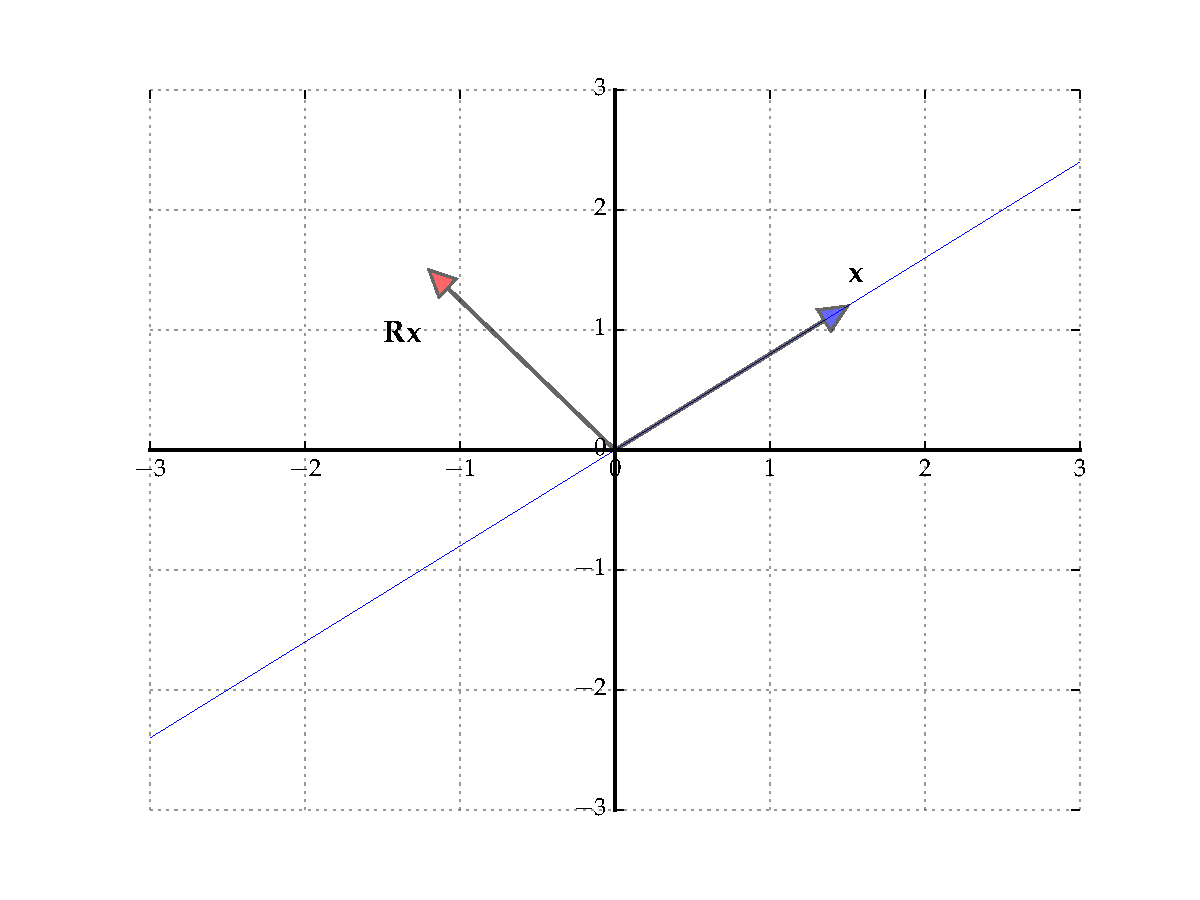
\includegraphics{rotation_1.pdf}}
        \caption{Матрица $\boldR$ поворачивает точки на $90^{\circ}$}
       \end{center}
    \end{figure}

\end{frame}


\begin{frame}
    \
    \vspace{2em}
    \begin{figure}
       \begin{center}
        \scalebox{.4}{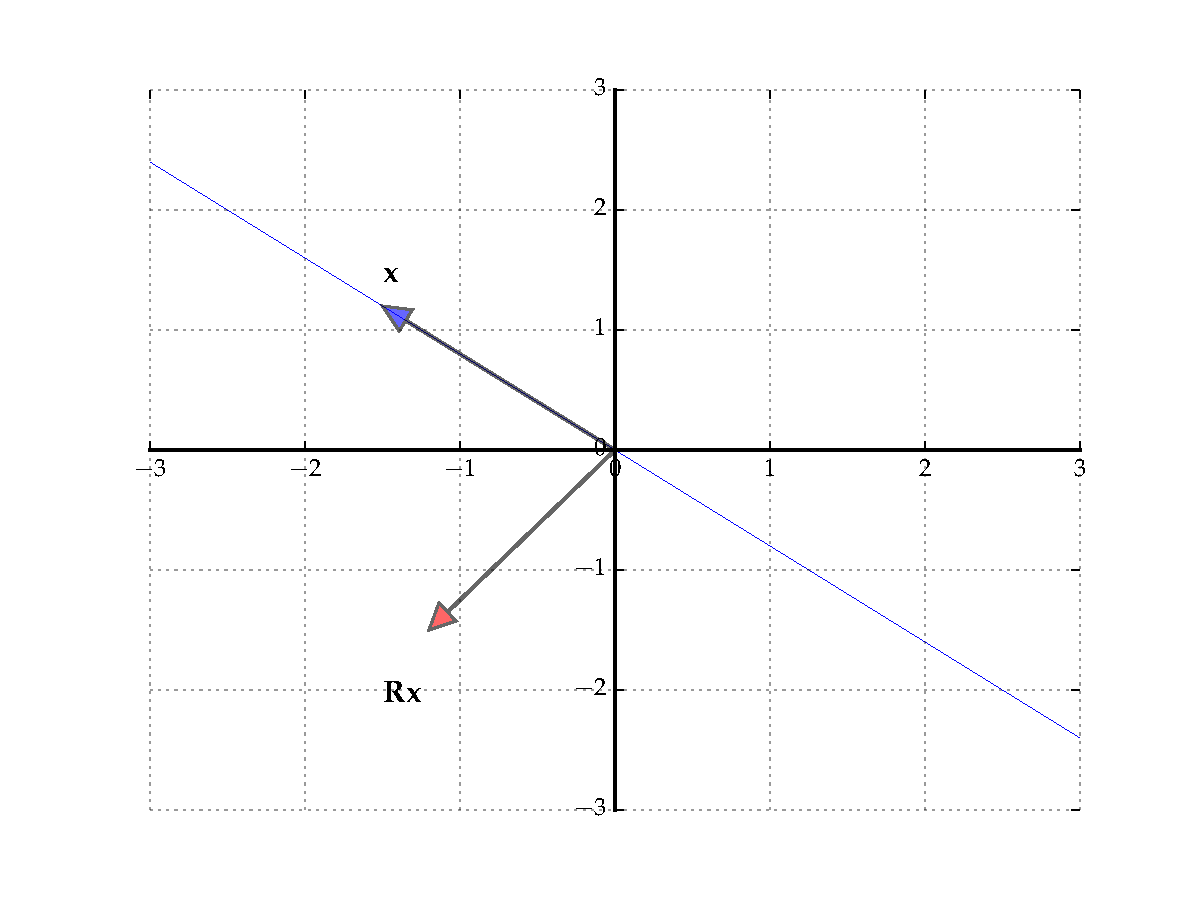
\includegraphics{rotation_2.pdf}}
        \caption{Матрица $\boldR$ поворачивает точки на $90^{\circ}$}
       \end{center}
    \end{figure}

\end{frame}

\begin{frame}
    
    \vspace{2em}
    Но $\boldR \boldx = \lambda \boldx$ может выполняться, \underline{если} мы 
    допускаем комплексные числа

    \vspace{1em}

    \Eg 
    %
    \begin{equation*}
        \left(
        \begin{array}{cc}
            0 & -1  \\
            1 & 0  \\
        \end{array}
        \right)
        \begin{pmatrix}
            1 \\
            -i
        \end{pmatrix}
        =
        \begin{pmatrix}
            i \\
            1
        \end{pmatrix}
        =
        i
        \begin{pmatrix}
            1 \\
            -i
        \end{pmatrix}
    \end{equation*}

    \vspace{.7em}
    То есть
    %
    \begin{equation*}
        \boldR \boldx = \lambda \boldx
        \quad \text{для} \quad
        \lambda := i
        \quad \text{и} \quad
        \boldx := 
        \begin{pmatrix}
            1 \\
            -i
        \end{pmatrix}
    \end{equation*}


    Тогда $(\boldx, \lambda)$ является собственной парой при условии, 
    что мы допускаем комплексные числа 

\end{frame}

\begin{frame}
    
    \vspace{2em}
    \Fact{\eqref{ET-fa:chei}} для любой квадратной матрицы $\boldA$ 
    %
    \begin{equation*}
        \lambda \text{ является собственным значением } \boldA \; \iff \;
        \det(\boldA - \lambda \boldI) = 0
    \end{equation*}
    %

    \vspace{1em}

    \Prf  Пусть $\boldA$ --- матрица размера $N \times N$ и $\boldI$ --- единичная 
    матрица размера $N \times N$

    Получается
    %
    \begin{align*}
        \det(\boldA - \lambda \boldI) = 0
        & \iff \boldA - \lambda \boldI \text{ сингулярно}
        \\
        & \iff \exists \, \boldx \not= \boldzero \st
            (\boldA - \lambda \boldI) \boldx = \boldzero
        \\
        & \iff \exists \, \boldx \not= \boldzero \st
        \boldA \boldx = \lambda \boldx
        \\
        & \iff \lambda 
        \text{ является собственным значением } \boldA
    \end{align*}

\end{frame}

\begin{frame}
    
    \vspace{2em}
    \Eg В случае матрицы $2 \times 2$,
    %
    \begin{equation*}
        \boldA =
        \left(
        \begin{array}{cc}
            a & b  \\
            c & d  \\
        \end{array}
        \right)
        \quad \implies \quad
        \boldA - \lambda \boldI =
        \left(
        \begin{array}{cc}
            a - \lambda & b  \\
            c & d - \lambda 
        \end{array}
        \right)
    \end{equation*}
    %
    \begin{align*}
        \fore
    \det(\boldA - \lambda \boldI) 
    & = (a - \lambda)(d - \lambda) - bc
    \\
    & = \lambda^2 - (a + d) \lambda + (ad - bc)
    \end{align*}
    
    Значит собственные значения $\boldA$ являются двумя корнями уравнения 
    %
    \begin{equation*}
        \lambda^2 - (a + d) \lambda + (ad - bc) = 0
    \end{equation*}
    
    Эквивалентно,
    %
    \begin{equation*}
        \lambda^2 - \trace(\boldA) \lambda + \det(\boldA) = 0
    \end{equation*}
    
\end{frame}


\begin{frame}

    \frametitle{Существование собственных значений}

    \vspace{2em}
    Возьмем матрицу $\boldA$ размера $N \times N$ 

    \vspace{0.5em}
    
    \Fact Существуют комплексные числа $\lambda_1, \ldots, \lambda_N$, такие что
    %
    \begin{equation*}
        \det(\boldA - \lambda \boldI) = \prod_{n=1}^N (\lambda_n - \lambda)
    \end{equation*}
    %

    Каждое такое $\lambda_i$ является собственным значением $\boldA$, потому что
    %
    \begin{equation*}
        \det(\boldA - \lambda_i \boldI) 
        = \prod_{n=1}^N (\lambda_n - \lambda_i) 
        = 0
    \end{equation*}
    %  
    Важно: не все собственные значения обязательно различны --- могут быть повторы

\end{frame}

\begin{frame}

     \vspace{2em}
    \Fact{\eqref{ET-fa:eiprop}} 
    %
    Возьмем матрицу $\boldA$ размера $N \times N$ с собственными значениями 
    $\lambda_1, \ldots, \lambda_N$. Получается
    %
    \begin{enumerate}
            \vspace{-0.6em}
        \item $\det(\boldA) = \prod_{n=1}^N \lambda_n$
            \vspace{0.4em}
        \item $\trace(\boldA) = \sum_{n=1}^N \lambda_n$
            \vspace{0.4em}
        \item если $\boldA$ симметрична, то $\lambda_n \in \RR$ для всех $n$
            \vspace{0.4em}
        \item если $\boldA$ несингулярна, то $\text{eigenvalues of } \boldA^{-1}
                = 1/\lambda_1, \ldots, 1/\lambda_N$
            \vspace{0.4em}
        \item если $\boldA = \diag(d_1, \ldots, d_N)$, то $\lambda_n = d_n$ для всех $n$
    \end{enumerate}

    \vspace{0.8em}
    %
    Значит матрица $\boldA$ несингулярна $\iff$ все ее собственные значения ненулевые
    
\end{frame}


\begin{frame}\frametitle{Квадратичные формы}

     \vspace{2em}
    Возьмем матрицу $\boldA$ размера $N \times N$ 
    
    \navy{Квадратичная функция} или \navy{квадратичная форма} в $\RR^N$, связанная с матрицей $\boldA$, --- это отображение $Q$, определяемое как
    %
    \begin{equation*}
        Q(\boldx) := \boldx^\T \boldA \boldx = \sum_{j=1}^N \sum_{i=1}^N a_{ij} x_i x_j
    \end{equation*}
    
    \vspace{.7em}
    \Eg Пусть $N = 2$ и $\boldA$ --- единичная матрица $\boldI$. Тогда
    %
    \begin{equation*}
        Q(\boldx) = \| \boldx \|^2 = x_1^2 + x_2^2
    \end{equation*}
    
\end{frame}

\begin{frame}
    
    \vspace{2em}
    \begin{figure}
   \begin{center}
    \scalebox{.45}{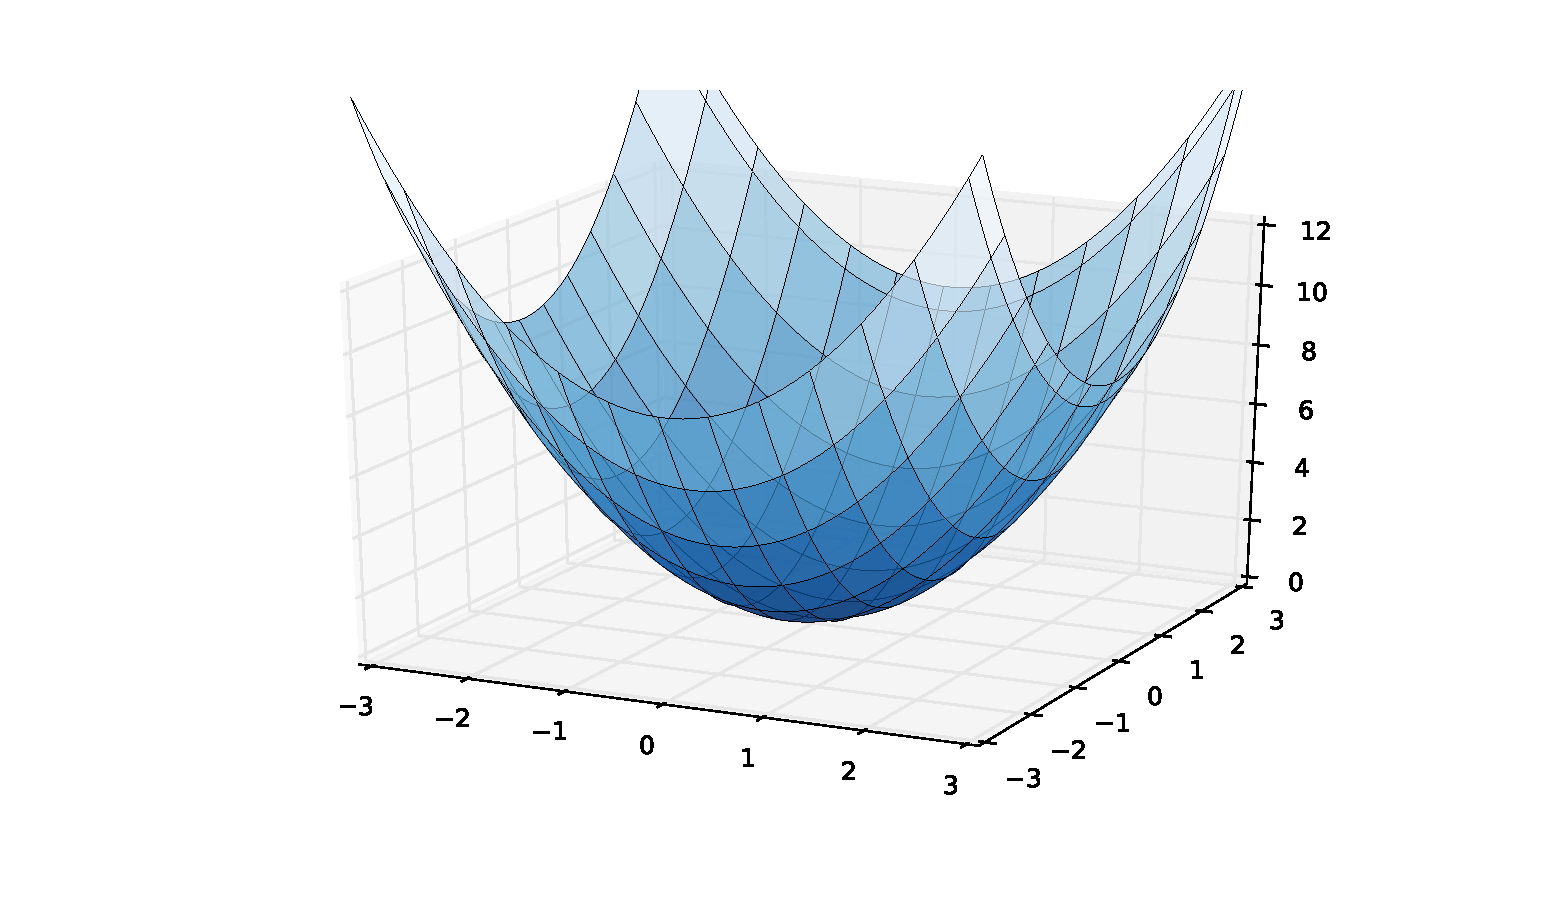
\includegraphics[trim={7.5em 2em 0 0em}, clip]{qform_pd.pdf}}
    \caption{\label{f:qform_pd} Квадратичная функция $Q(\boldx) = x_1^2 + x_2^2$ }
   \end{center}
    \end{figure}

\end{frame}

\begin{frame}

    \vspace{2em}
    Внимание:
    \begin{itemize}
        \item График для $Q(\boldx) = \| \boldx \|^2 = x_1^2 + x_2^2$ лежит всюду выше нуля
    \end{itemize}
    
    \vspace{.7em}
    Матрица $\boldA$ с квадратичной формой с указанным выше свойством $Q(\boldx) \geq 0$  называется \emph{положительно определенной}
    
\end{frame}

\begin{frame}

    \vspace{2em}
    В более общем смысле, симметричная матрица $\boldA$ размера $N \times N$ называется
    %
    \begin{itemize}
        \item \navy{неотрицательно определенной}, если $\boldx^\T \boldA \boldx \geq 0$
            для всех $\boldx \in \RR^N$, 
        \item \navy{положительно определенной}, если $\boldx^\T \boldA \boldx > 0$ для всех $\boldx \in \RR^N$ with $\boldx \not= \boldzero$,
        \item \navy{неположительно определенной}, если $\boldx^\T \boldA \boldx \leq 0$
            для всех $\boldx \in \RR^N$, и
        \item \navy{отрицательно определенной}, если $\boldx^\T \boldA \boldx < 0$ для всех $\boldx \in \RR^N$ with $\boldx \not= \boldzero$.
    \end{itemize}
    
    \vspace{.7em}
    Если $\boldA$ не подходит ни к одной из этих категорий, то $\boldA$ называется \navy{неопределенной}
    
\end{frame}

\begin{frame}

     \vspace{2em}
    \begin{figure}
   \begin{center}
    \scalebox{.45}{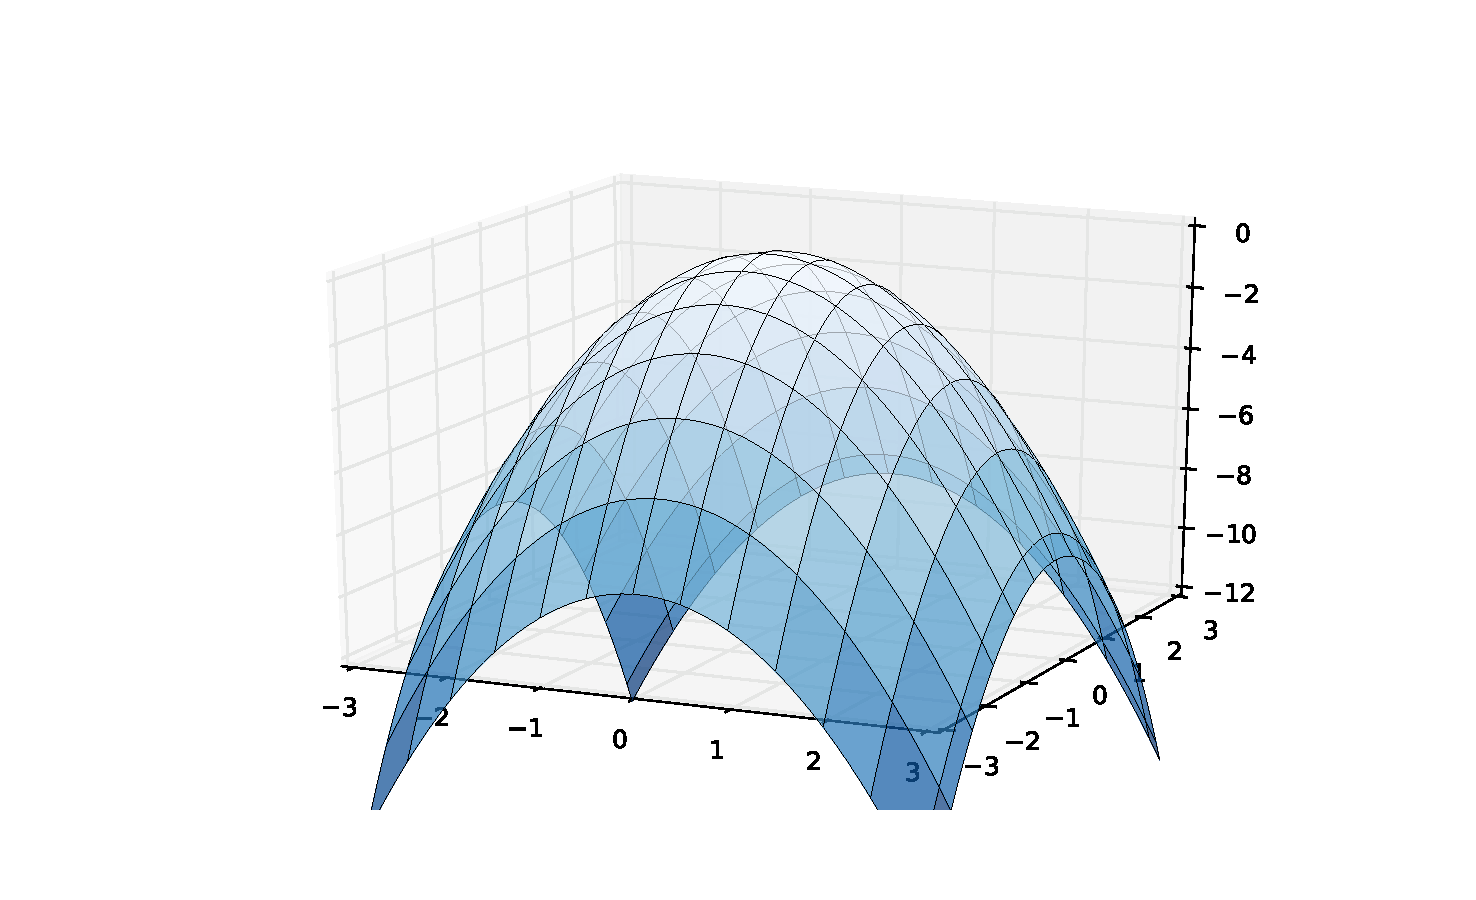
\includegraphics[trim={5em 2em 0 2em}, clip]{qform_nd.pdf}}
    \caption{\label{f:qform_nd} Квадратичная функция $Q(\boldx) = -x_1^2 - x_2^2$ }
   \end{center}
    \end{figure}
    
\end{frame}

\begin{frame}

     \vspace{2em}
    \begin{figure}
   \begin{center}
    \scalebox{.4}{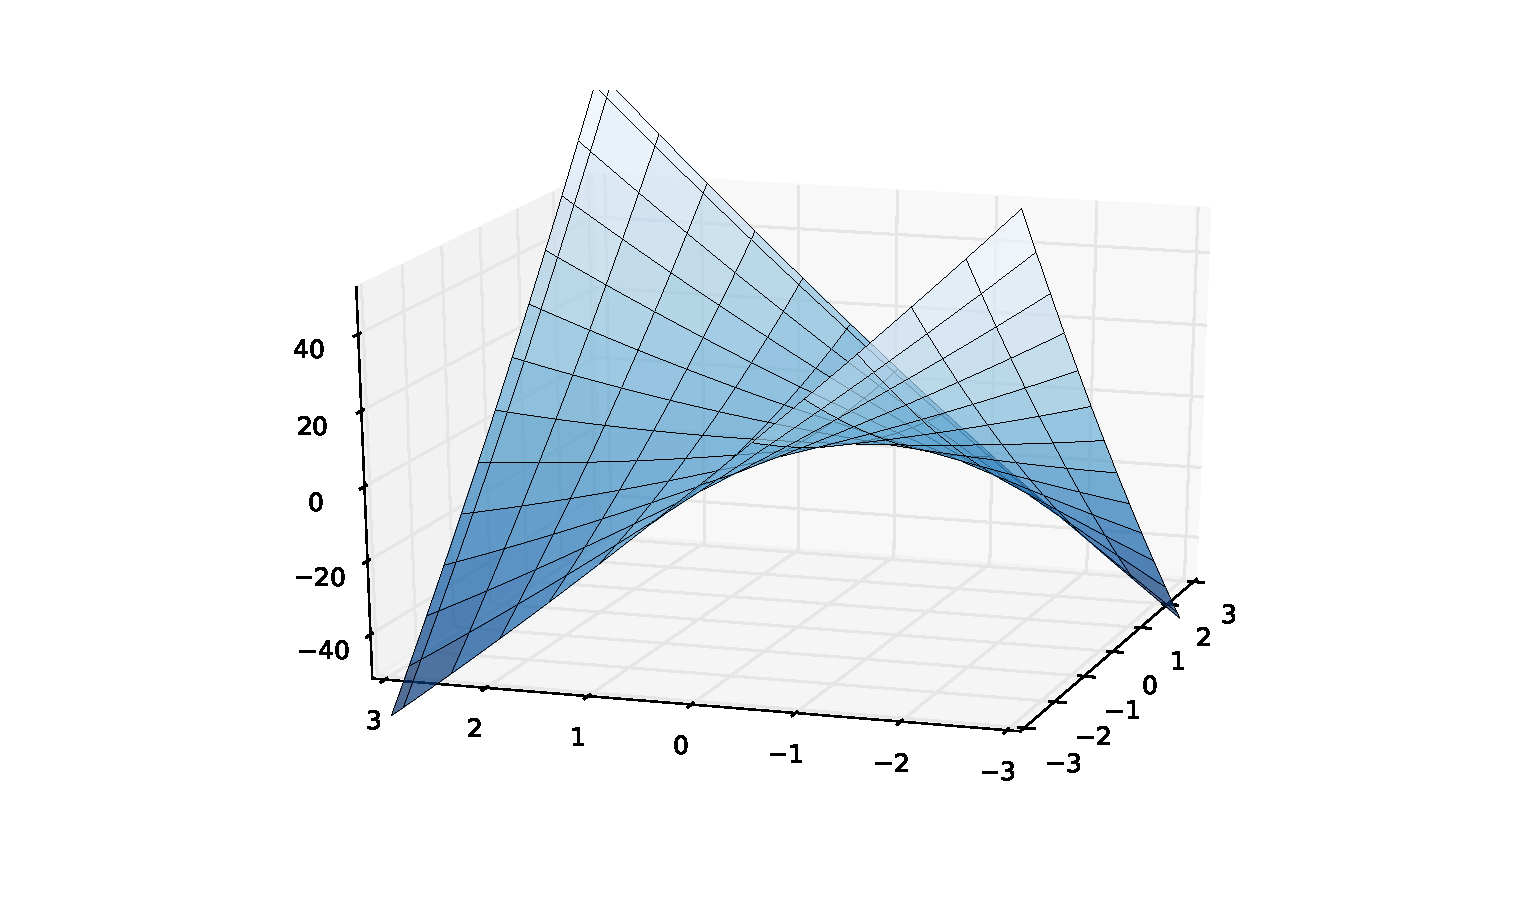
\includegraphics[trim={5em 2em 2em 2em}, clip]{qform_indef.pdf}}
    \caption{\label{f:qform_indef} Квадратичная функция $Q(\boldx) = x_1^2/2 +
        8 x_1 x_2 + x_2^2/2$ }
   \end{center}
    \end{figure}
    
\end{frame}

\begin{frame}  

   \vspace{2em}
    Когда матрица $\boldA$ диагональная: 
    %   
    \begin{equation*}
        \boldA = \diag(d_1, \ldots, d_N)
        \quad \text{подразумевает} \quad
        Q(\boldx) = d_1 x_1^2 + \cdots + d_N x_N^2  
    \end{equation*}
    
    
    \vspace{.7em}
    Диагольная матрица положительно определена, тогда и только тогда, когда 
    все диагональные элементы положительны
    
\end{frame}

\begin{frame}

    \vspace{2em}
    \Fact{\eqref{ET-fa:eigdef}}
    Пусть $\boldA$ --- некоторая симметричная матрица. Матрица $\boldA$ 
    %
    \begin{enumerate}
        \item положительна определена тогда и только тогда, когда все ее собственные значения положительны
        \item отрицательно определена тогда и только тогда, когда все ее собственные значения отрицательны
    \end{enumerate}
    %
    ...аналогично для неположительно и неотрицательно определенных
    
    \vspace{.7em}
    \Fact{\eqref{ET-fa:ipde}}
        Если $\boldA$ положительно определена, то $\boldA$ несингулярна, $\det \boldA > 0$

\end{frame}

\begin{frame}

     \vspace{2em}
    Необходимое (но не достаточное) условие для каждого вида определенности:
    
    \vspace{.7em}
    \Fact{\eqref{ET-fa:ipde0}}
        Если $\boldA$ положительна определена, то
        каждый элемент $a_{nn}$ на главной диагонали положительный, то же самое для
        неотрицательной, неположительной и отрицательной.
        
\end{frame}

\section{Проекция и разложение}

\begin{frame}\frametitle{Матрицы проекции}

     \vspace{2em}
    Напомним, что для любого подпространства $\mathbb{R}^{N}$, $S$, соответствующая 
    проекция $\boldP = \proj S$ является линейным отображением из $\RR^N$ в $\RR^N$

    \vspace{.7em}
    Вспомним теорему~\ref{ET-t:lmaeq}: существует матрица $\hat \boldP$ размера 
    $N \times N$, такая что $\boldP \boldx =
    \hat \boldP \boldx$ для всех $\boldx \in \RR^N$
    %
    \begin{itemize}
        \item с этого момента $\boldP$ также будет означать соответствующую матрицу
    \end{itemize} 
    
    Как выглядит эта матрица?
    
\end{frame}

\begin{frame}

     \vspace{.7em}
    \Thm {\eqref{ET-t:projon}}
    Пусть $S$ --- подпространство в $\RR^N$. Если $\boldP = \proj S$, то
    %
    \begin{equation}
        \label{eq:projb}
        \boldP = \boldB (\boldB^\T\boldB)^{-1} \boldB^\T  
    \end{equation}
    %
    для каждой матрицы $\boldB$, такой что столбцы $\boldB$ формируют базис $S$ 
    
    \vspace{.7em}
    Смотрите упражнение~\ref{ET-ex:projon} для доказательства
    
    \begin{itemize}
        \item  Матрица $\boldM = \boldI -
                \boldP$ обозначает остаточную проекцию (смотрите 
                страницу~\pageref{ET-eq:ann0})
    \end{itemize}
    
\end{frame}

\begin{frame}
    
    \vspace{2em}
    \Eg
    Вспомним пример~\ref{ET-eg:pvones} на странице~\pageref{ET-eg:pvones}
    
    Мы выяснили, что проекция $\boldy \in \RR^N$ на $\Span\{\boldone\}$ --- это
    $\bar y \boldone$
    
    Тот же результат с помощью теоремы~\eqref{ET-t:projon}:
    \begin{itemize}
        \item Так как $\boldone$ является базисом $\Span\{\boldone\}$:
            %
            \begin{equation*}
                \label{eq:pcz}
                \boldP = \proj \; \Span\{\boldone\} 
                \; \implies \;
                \boldP 
                = \boldone (\boldone^\T\boldone)^{-1} \boldone^\T  
                = \frac{1}{N} \boldone \boldone^\T  
            \end{equation*}
        %
        \item Значит, $\boldP \boldy = \bar y \boldone$, как и ожидалось
        \item Соответствующая остаточная проекция
        %
        \begin{equation*}
            \label{eq:pczm}
            \boldM_c
            = \boldI - \frac{1}{N} \boldone \boldone^\T  
        \end{equation*}
    \end{itemize}

\end{frame}

\begin{frame}

     \vspace{2em}
    \Fact{\eqref{ET-fa:anox}} 
    По постановке теоремы~\ref{ET-t:projon}, получается 
    %
    \begin{enumerate}
        \item $\boldM \boldB = \boldzero$
        \item $\boldP \boldB = \boldB$
    \end{enumerate}
    
    Докажите в качестве упражнения (упр. \ref{ET-ex:anox} в ET)
    
    \vspace{1em}
    Легко заметить, что $\boldM_c$ в предыдущем примере отображает
    $\boldone$ в $\boldzero$
    
\end{frame}

\begin{frame}
    
    \vspace{2em}
    Квадратная матрица $\boldA$ является \navy{иденпотентной}, 
    если $\boldA \boldA = \boldA$ 
    
    \vspace{.7em}
    \Fact{\eqref{ET-fa:pmsi}}
        И $\boldP$, и $\boldM$ симметричны и иденпотентны
    
    (Упражнение: проверьте прямыми вычислениями)
    
    \vspace{.7em}
    Интуиция: проецирование
    на подпространство дважды --- это то же самое, что проецировать один раз -- вспомните 
    факт~\ref{ET-fa:opt3} на странице~\pageref{ET-fa:opt3}
    
\end{frame}

\begin{frame}
    
    \vspace{2em}
    \Fact{\eqref{ET-fa:trop}}
    Пусть $S$ является линейным подпространством в $\RR^N$. Если $\boldP = \proj S$ и 
    $\boldM$ --- остаточная проекция, то
    %
    \begin{enumerate}
        \item $\rank \boldP  = \trace \boldP  = \dim S$ и
        \item $\rank \boldM  = \trace \boldM  = N - \dim S$
    \end{enumerate}
  
  
    \Prf
    \begin{itemize}
        \item Ранг линейного отображения --- это размерность его диапазона.  Когда $\boldP = \proj S$, Диапазон
            $\boldP$ равняется $S$
        \item Чтобы показать, что $\trace \boldP = \dim S$ также соблюдается, используем 
        факт~\ref{ET-fa:idtrra}--  $\trace\boldP
                = \dim S$, 
        \item Это следует из того, что $\trace\boldM = N - \dim S$, потому что
            %
            \begin{equation*}
                \trace\boldM 
                = \trace(\boldI - \boldP) 
                = \trace \boldI - \trace\boldP 
                = N - \dim S
            \end{equation*}

    \end{itemize}
  
\end{frame}


\begin{frame}\frametitle{Переопределенные системы уравнений}
    
    \vspace{2em}
    Рассмотрим систему уравнений в виде $\boldA \boldx = \boldb$, когда:
    \begin{itemize}
        \item Матрица $\boldA$ размера
        $N \times K$ имеет полный ранг столбцов
        \item Вектор $\boldx$ имеет размер $K\times1$
        \item Вектор $\boldb$ имеет размер $N\times 1$ 
        \item $K\leq N$
    \end{itemize} 
    
    \vspace{1em}
    Принимая как данность $\boldA$ и $\boldb$, мы ищем $\boldx \in \RR^K$, такой что
    $\boldA \boldx = \boldb$

\end{frame}

\begin{frame}

     \vspace{2em}
    Если $K = N$, то система имеет ровно одно решение
    
    \vspace{1em}
    Когда $N > K$, система уравнений считается \navy{переопределенной}:
    %
    \begin{itemize}
        \item количество уравнений $>$ количества неизвестных
        \item количество ограничений $>$ количества степеней свободы
    \end{itemize}
    
    Возможно, не удастся найти $\boldb$, который удовлетворяет всем $N$ уравнениям
    
\end{frame}

\begin{frame}

     \vspace{2em}
    Вспомним линейное отображение $T \colon
    \RR^K \to \RR^N$, где $T\boldx = \boldA \boldx$
    
    \vspace{1em}
    Следующие утверждения эквивалентны:
    %
    \begin{enumerate}
        \item существует $\boldx \in \RR^K$, такой что $\boldA \boldx = \boldb$
        \item вектор $\boldb \in \colspace \boldA$
        \item вектор $\boldb \in \range T$
    \end{enumerate}
    
     \vspace{.7em}
    Теорема~\ref{ET-t:lfoc} на странице~\pageref{ET-t:lfoc}: когда $K <
    N$, функция $T$ не может быть сюръекцией -- возможные $\boldb$ находятся
    вне диапазона $T$
    
\end{frame}

\begin{frame}

     \vspace{2em}
    Когда $K < N$, случай с $\boldb \in
    \colspace \boldA$ является ``очень редким``, потму что:
    %
    \begin{itemize}
        \item точка $\boldb$ является произвольной точкой в $\RR^N$
        \item пространство $ \colspace \boldA$ имеет размерность $K$
        \item подпространста $\RR^N$ с размерностями $K$ имеют
        ``нулевую меру Лебега'' -- ``шанс'' того, что $\boldb$ лежит в 
        этом подпространстве, крошечный
    \end{itemize}
    
\end{frame}

\begin{frame}

     \vspace{2em}
    Стандартный подход: признать, что точного решения может не существовать
    
    \vspace{1em}
    Следует сосредоточиться на поиске $\boldx \in \RR^K$, чтобы $\boldA
    \boldx$ оказалось настолько близко к $\boldb$, насколько возможно
    \begin{itemize}
        \item близки по обычной Евклидовой норме
    \end{itemize}
    
    \vspace{1em}
    Задача минимизации называется \navy{методом наименьших квадратов}
    %
    \begin{equation}
        \label{eq:mxls}
        \hat{\boldx} \colon = \argmin_{\boldx \in \RR^K} \| \boldb - \boldA \boldx \|
    \end{equation}
    
\end{frame}


\begin{frame}

     \vspace{2em}
    При условии, что $\boldA$ размера $N \times K$ с $K \leq N$ и 
    $\boldb$ размера $N \times 1$, 
    мы можем использовать теорему ортогональной проекции для решения \eqref{eq:mxls}
    
    \vspace{.7em}
    \Thm{\eqref{ET-t:lssol}}
        Если $\boldA$ имеет полный ранг столбцов, то \eqref{eq:mxls} имеет 
        единственное решение
        %
        \begin{equation}
            \label{eq:dlse}
            \hboldx := (\boldA^\T \boldA)^{-1} \boldA^\T \boldb
        \end{equation}
        %
    \end{frame}
    
\begin{frame}

    \vspace{2em}
    \Prf 
    
    Пусть:
    %
    \begin{itemize}
        \item $\boldA$ и $\boldb$ be as in the statement of the theorem
        \item $\hboldx$ be as in \eqref{eq:dlse} и
        \item $S := \colspace \boldA$
    \end{itemize}
    %
    By full column rank assumption, the columns of $\boldA$ form a basis for
    $S$. Applying theorem~\ref{ET-t:projon}, orthogonal projection of $\boldb$
    onto $S$ is 
    %
    \begin{equation}
        \label{eq:ibprojon}
        \boldP\boldb 
        := \boldA (\boldA^\T \boldA)^{-1} \boldA^\T \boldb  
         = \boldA \hboldx
    \end{equation}
    
    Since the orthogonal projection theorem gives a unique
    minimizer in terms of the closest point in $S$ to $\boldb$,
    %
    \begin{equation}
        \label{eq:sfy}
        \| \boldb - \boldA\hboldx \| < \| \boldb - \boldy\|
        \quad \text{для всех } \boldy \in S, \; \boldy \not= \boldA \hboldx
    \end{equation}

\end{frame}
    
\begin{frame}
    
    \vspace{2em}
    \Prf (cont.) Pick any $\boldx \in \RR^K$ , такая что $\boldx \not= \hboldx$
    
    We have $\boldA \boldx \in S$
    
    In addition, since $\boldx \not= \hboldx$, и since $\boldA$ has full column
    rank, it must be that $\boldA \boldx \not= \boldA \hboldx$
    (ex.~\ref{ET-ex:ui})
    
     \vspace{.7em}
    Hence
    %
    \begin{equation*}
        \| \boldb - \boldA\hboldx \| < \| \boldb - \boldA \boldx\|
        \quad \text{для всех } \boldx \in \RR^K, \; \boldx \not= \hboldx
    \end{equation*}
    %
    In other words, $\hboldx$ is the unique solution to \eqref{eq:mxls}
    
\end{frame}

\begin{frame}

    \vspace{2em}
    In  \eqref{eq:dlse}, the matrix $(\boldA^\T\boldA)^{-1} \boldA^\T$ 
    называется the \navy{pseudoinverse} of $\boldA$ 
    
    \vspace{1em}
    если $K =
    N$, then the
    least squares solution $\hboldx$ in \eqref{eq:dlse} reduces to:
    %
    \begin{equation*}
        \boldx = \boldA^{-1}\boldb
    \end{equation*}
    
\end{frame}

\begin{frame}

     \vspace{2em}
    What happens если the columns of $\boldA$ are not
    linearly independent? 
    
    \begin{itemize}
        \item   the set $\colspace \boldA$ is still a linear
        subspace и the orthogonal projection theorem still gives us a closest
        point $\boldP \boldb$ to $\boldb$ in $\colspace \boldA$
        \item   since $\boldP
        \boldb \in \colspace \boldA$, there still exists a vector $\hboldx$ such
        that $\boldP \boldb = \boldA \hboldx$
        \item    but there
        exists an infinity of such vectors
    \end{itemize}
    
    See Exercise~\ref{ET-ex:lsiosol}
    
\end{frame}


\section{Diagonalisation и Spectral Theory} 

\begin{frame}\frametitle{QR Decomposition}

     \vspace{2em}
    The \navy{QR decomposition} of a given matrix $\boldA$ is a product of the form $\boldQ \boldR$
    \begin{itemize}
        \item first matrix has orthonormal columns и 
        \item the second is upper triangular
    \end{itemize}
    
    \vspace{1em}
    Applications include least squares problems и the computation of eigenvalues
    
\end{frame}

\begin{frame}

     \vspace{2em}
    \Thm{\eqref{ET-t:qr}}
    если $\boldA$ is an $N \times K$ matrix with full column rank, then there exists a
    factorization $\boldA = \boldQ \boldR$ where
    %
    \begin{enumerate}
        \item $\boldR$ is $K \times K$, upper triangular и nonsingular, и 
        \item $\boldQ$ is $N \times K$, with orthonormal columns
    \end{enumerate}
    %
    See page~\pageref{ET-t:qr} in ET for a proof
    
\end{frame}

\begin{frame}

     \vspace{2em}
    Given the decomposition $\boldA = \boldQ \boldR$, the least squares solution
    $\hboldx$ defined in \eqref{eq:dlse} can also be written as:
    $$\hboldx =
    \boldR^{-1} \boldQ^\T \boldb$$
    
    See Ex.~\ref{ET-ex:qrlsq}
    
    \vspace{.7em}
    Premultiplying by $\boldR$:
    $$\boldR \hboldx = \boldQ^\T \boldb$$
    
\end{frame}

\begin{frame}\frametitle{Diagonalisation и Spectral Theory}

     \vspace{2em}
    если $f \colon A \to A$ и $g \colon B \to B$, then
    $g$ is said to be \navy{topologically conjugate} to $f$ whenever there exists
    a continuous bijection $\tau \colon B \to A$ , такая что $$f = \tau \circ g \circ
    \tau^{-1}$$
    
    \vspace{.7em}
    Can be beneficial если $g$ is somehow simpler
    than $f$
    
\end{frame}

\begin{frame}

    \vspace{2em}
    A square matrix $\boldA$ is said to be \navy{similar} to another matrix $\boldB$ если there exists an invertible matrix $\boldP$ , такая что $\boldA = \boldP \boldB \boldP^{-1}$

    \begin{figure}
   \begin{center}
    \begin{tikzpicture}[scale=1,
    axis/.style={->, >=stealth'},
    important line/.style={thick},
    dashed line/.style={dashed, thin},
    every node/.style={color=black},
    decoration={brace,amplitude=7pt},
    ] 

%% draw nodes
\coordinate (x1) at (-2,2);  \coordinate (x11) at (-2,1.8); \coordinate (x12) at (-1.8,2);  
\coordinate (x2) at (-2,0); \coordinate (x21) at (-1.8,0); \coordinate (x22) at (-2,0.2);
\coordinate (x3) at (2,2);   \coordinate (x31) at (1.8,2);  \coordinate (x32) at (2,1.8);
\coordinate (x4) at (2,0);  \coordinate (x41) at (1.8,0); \coordinate (x42) at (2,0.2);

\node[fill=black,circle,scale=0.37] at (x1){};
\node[fill=black,circle,scale=0.37] at (x2){};
\node[fill=black,circle,scale=0.37] at (x3){};
\node[fill=black,circle,scale=0.37] at (x4){};

%% label x & Ax
\draw (x2) node[below=5pt] {$\boldx$};
\draw (x4) node[below=5pt] {$\boldA\boldx$};

%% draw arrows
\draw[important line, ->]  (x21) -- node[above=5pt] {$\boldA$} (x41);
\draw[important line, ->]  (x22) -- node[left=5pt] {$\boldP^{-1}$} (x11);
\draw[important line, ->]  (x12) -- node[above=5pt] {$\boldB$} (x31);
\draw[important line, ->]  (x32) -- node[right=5pt] {$\boldP$} (x42);
  
\end{tikzpicture}

    \caption{\label{f:diagonalize} $\boldA$ is similar to $\boldB$}
   \end{center}
    \end{figure}
    
\end{frame}

\begin{frame}
   
    \vspace{2em}
    если $\boldA$ is similar to a diagonal matrix, then $\boldA$ is
    called \navy{diagonalizable}
    
    \vspace{.7em}
    We are interested in similarity to simple matrices, и diagonal matrices are the simplest kind 
    
\end{frame}

\begin{frame}

     \vspace{2em}
    \Fact{\eqref{ET-fa:powsm}}
        если $\boldA$ is similar to $\boldB$, then $\boldA^t$ is similar to
        $\boldB^t$ для всех $t \in \NN$
    
    \vspace{.7em}
    \Eg
    We want to calculate $\boldA^t$ for some given $t \in \NN$ 
    
    если $\boldA = \boldP \boldLambda \boldP^{-1}$ for some
    $\boldLambda = \diag(\lambda_1, \ldots, \lambda_N)$, then by
    fact~\ref{ET-fa:powsm} и fact~\ref{ET-fa:powdm}, we
    have
    %
        $$\boldA^t = \boldP \diag(\lambda_1^t, \ldots, \lambda_N^t)
        \boldP^{-1}$$
    
\end{frame}

\begin{frame}\frametitle{Diagonalization и Eigenvalues}

    \vspace{.7em}
    \Fact{\eqref{ET-fa:diagee}}
    если $\boldA = \boldP \boldLambda \boldP^{-1}$ for some $\boldLambda =
        \diag(\lambda_1, \ldots, \lambda_N)$, then $(\col_n \boldP,
            \lambda_n)$ is an eigenpair of $\boldA$ for each $n$
            
    \vspace{.7em}    
    
    \Prf
    Observe $\boldA
    = \boldP \boldLambda \boldP^{-1}$ implies $\boldA \boldP = \boldP \boldLambda$
    
    Equating the $n$th column on each side gives 
    %
        $$\boldA \boldp_n = \lambda_n
        \boldp_n$$
    %
    Where $\boldp_n := \col_n \boldP$
    
    Note  $\boldp_n$ is not the
    zero vector because $\boldP$ is invertible
        
\end{frame}

\begin{frame}
    
    \vspace{2em}
    But when is $\boldA$ diagonalizable?  
    
    \vspace{.7em}
    \Fact (3.3.7)
    An $N \times N$ matrix $\boldA$ is diagonalizable если и only если
    it has $N$ linearly independent eigenvectors

\end{frame}


\begin{frame}

     \vspace{2em}
    In some cases, we can get an even simpler matrix decomposition если 
    the matrix $\boldP$ has orthogonal columns 

    These kinds of matrices are called \navy{orthogonal matrices}
    
    \vspace{.7em}
    \Fact{\eqref{ET-fa:orthmat}}
    если $\boldQ$ и $\boldP$ are $N \times N$ orthogonal matrices, then
    %
    \begin{enumerate}
        \item $\boldQ^\T$ is orthogonal и $\boldQ^{-1} = \boldQ^\T$,
        \item $\boldQ \boldP$ is orthogonal, и
        \item $\det \boldQ \in \{-1, 1\}$.
    \end{enumerate}
    
\end{frame}
    
\begin{frame}

    \vspace{2em}
    если $\boldA = \boldQ \boldLambda \boldQ^{-1}$ и $\boldQ$ has orthonormal columns,
    then $$\boldA = \boldQ \boldLambda \boldQ^\T$$
    
    Clearly, $\boldA$ must be symmetric. Next theorem shows symmetry of $\boldA$ is also sufficient
    
    \vspace{.7em}
    \Thm{\eqref{ET-t:dismat}}
    если $\boldA$ is symmetric, then $\boldA$ can be
    diagonalized as $\boldA = \boldQ \boldLambda \boldQ^\T$, where 
    $\boldQ$ is an orthogonal matrix и $\boldLambda$ is the 
    diagonal matrix formed from the eigenvalues of $\boldA$
    
\end{frame}

\begin{frame}

   \vspace{2em}

    Above theorem was a version of the \navy{spectral decomposition theorem}

    $\boldQ \boldLambda \boldQ^\T$ называется the \navy{symmetric eigenvalue
    decomposition} of $\boldA$\ -- action of $\boldA$ on an
    $N \times 1$ vector $\boldx$:
    %
    \begin{equation*}
        \boldA\boldx = \sum_{n=1}^N \lambda_n (\boldu_n^\T \boldx) \boldu_n
    \end{equation*}
    %
    where $\lambda_n$ is the $n$th eigenvalue of $\boldA$ и $\boldu_n = \col_n \boldQ$
    
    \vspace{.7em}
    Compare with $\boldx = \sum_{n=1}^N (\boldu_n^\T \boldx) \boldu_n$
    
\end{frame}

\begin{frame}

    \vspace{2em}
    \Fact{\eqref{ET-fa:sqrtsnd}}
    если $\boldA$ is nonnegative definite, then $\sqrt{\boldA}$
    exists и equals $\boldQ \sqrt{\boldLambda} \boldQ^\T$.
    The matrix $\sqrt{\boldLambda}$ is given by $\diag(\sqrt{\lambda_1},
    \ldots, \sqrt{\lambda_N})$
    
    \vspace{.7em}
    \Fact{\eqref{ET-fa:cholesky}}
    если $\boldA$ is positive definite, then there exists a nonsingular, upper
    triangular matrix $\boldR$ , такая что $\boldA = \boldR^\T \boldR$
    
    This decomposition называется the \navy{Cholesky decomposition}

\end{frame}

\begin{frame}

    \vspace{2em}
    \Prf (Cholesky decomposition)
    We can write:
    %
        \begin{equation*}
            \boldA 
            = \boldQ \boldLambda \boldQ^\T
            = \boldQ \sqrt{\boldLambda} \sqrt{ \boldLambda} \boldQ^\T
            = (\sqrt{ \boldLambda} \boldQ^\T)^\T \sqrt{ \boldLambda} \boldQ^\T
        \end{equation*}
    %
    Then apply the QR decomposition to $\sqrt{ \boldLambda} \boldQ^\T$:
    %
        $$\sqrt{ \boldLambda} \boldQ^\T = \tilde \boldQ \boldR$$
    %
    where $\boldR$ is nonsingular и upper triangular, и $\tilde \boldQ$ has
    orthonormal columns
    
    \vspace{.7em}
    Because the columns of $\tilde \boldQ$ are orthonormal,
    %
        \begin{equation*}
        \boldA 
        = (\tilde \boldQ \boldR)^\T \tilde \boldQ \boldR
        =  \boldR^\T \tilde \boldQ^\T \tilde \boldQ \boldR
        =  \boldR^\T \boldR
        \end{equation*}
    
\end{frame}


\begin{frame}

    \vspace{2em}
    \frametitle{Norms и Continuity}
    
    Given vector sequence $\{\boldx_n\}$ in $\RR^K$ и any point $\boldx \in \RR^K$, we say that $\{\boldx_n\}$ \navy{converges} to $\boldx$ и write
    \navy{$\boldx_n \to \boldx$} если, для любых $\epsilon > 0$, there exists an $N
    \in \NN$ , такая что $\|\boldx_n - \boldx\| < \epsilon$ whenever $n \geq N$
    
    \vspace{.7em}
    Equivalently, the real-valued sequence $z_n := \|\boldx_n - \boldx\|$
    converges to zero in $\RR$ as $n \to \infty$

\end{frame}

\begin{frame}
    
    \vspace{2em}
    \Fact (3.3.11)
    The following results hold:
    %
    \begin{enumerate}
        \item если $\boldx_n \to \boldx$ и $\boldy_n \to \boldy$, then $\boldx_n +
            \boldy_n \to \boldx +  \boldy$.
        \item если $\boldx_n \to \boldx$ и $\alpha \in \RR$, then $\alpha \boldx_n 
            \to \alpha \boldx$.
        \item $\boldx_n \to \boldx$ если и only если $\bolda^\T \boldx_n \to
            \bolda^\T \boldx$ для всех $\bolda \in \RR^K$.
    \end{enumerate}


\end{frame}

\begin{frame}

    \vspace{2em}
    We want to extend notion of convergence to matrices
    
    \vspace{.7em}
    The \navy{matrix norm} of $N \times K$ matrix $\boldA$:
    %
    \begin{equation}
    \label{eq:mn}
    \| \boldA \| :=
    \max \left\{ 
        \| \boldA \boldx \| \,: \, 
        \boldx \in \RR^K, \; \| \boldx \| = 1
        \right\}
    \end{equation}

    \vspace{.7em}
    The value of the matrix norm is not easy to solve for in
    general
    
    However, the matrix
    norm behaves like the vector norm
    
\end{frame}

\begin{frame}

    \vspace{2em}
    \Fact (3.3.12)
    для любых conformable matrices $\boldA$ и $\boldB$, the matrix norm 
    satisfies
    %
    \begin{enumerate}
        \item $\| \boldA \| \geq 0$ и $\| \boldA \| = 0$ если и only если all entries of
            $\boldA$ are zero,
        \item $\| \alpha \boldA \| = |\alpha| \| \boldA \|$ для любых scalar
            $\alpha$,
        \item $\| \boldA + \boldB \| \leq \| \boldA \| + \| \boldB \|$, и
        \item $\| \boldA \boldB \| \leq \| \boldA \| \| \boldB \|$.
    \end{enumerate}
    
    
\end{frame}

\begin{frame}

    \vspace{2em}
    \Fact{\eqref{ET-fa:mnbd}}
    для любых $J \times K$ matrix $\boldA$ with elements $a_{jk}$, we have
    %
    \begin{equation*}
        \| \boldA \| \leq \sqrt{JK} \max_{jk} |a_{jk}|
    \end{equation*}
    
    \vspace{1em}
    если every element of
    $\boldA$ is close to zero then $\| \boldA \|$ is also close to zero

\end{frame}

\begin{frame}\frametitle{Neumann Series}

    \vspace{2em}
    Later on, we study dynamic systems of the form
    %
        $$\boldx_{t+1} = \boldA \boldx_t + \boldb$$
    %
    
    \vspace{.7em}
    Does there exist a ``stationary" vector
  $\boldx \in \RR^N$, in the sense that $\boldx_t = \boldx$ implies $\boldx_{t+1} =
  \boldx$?
  
    We seek an $\boldx \in \RR^N$ that solves the
    system of equations
    %
    \begin{equation}
        \label{eq:lpfde}
        \boldx = \boldA \boldx + \boldb 
        \qquad (\boldA \text{ is } N \times N \text{ и } \boldb \text{ is } N
        \times 1)
    \end{equation}
    
\end{frame}

\begin{frame}
    
    \vspace{2em}
    Рассмотрим the scalar case $x = a x + b$
    
    \vspace{.7em}
    если $|a| < 1$, then there is a unique solution
    %
    \begin{equation*}
        \bar x 
        = \frac{b}{1-a} 
        = b \sum_{k=0}^{\infty} a^k 
    \end{equation*}
 
    \vspace{.7em}
    The Neumann series Lemma helps generalise to $\mathbb{R}^{N}$
    
    \vspace{1em}
    \Thm{\eqref{ET-t:nms}}
    если $\boldA$ is square и $\| \boldA^j \| < 1$
    for some $j \in \NN$, then $\boldI - \boldA$ is invertible, и
    %
    \begin{equation*}
        \label{eq:nmse}
        (\boldI - \boldA)^{-1} = \sum_{i=0}^{\infty} \boldA^i 
    \end{equation*}
    
\end{frame}
 
\begin{frame}

    \vspace{.7em}
    When the condition of the Neumann series lemma holds, \eqref{eq:lpfde}
    has the unique solution
    %
    \begin{equation*}
        \bar \boldx 
        = (\boldI - \boldA)^{-1} \boldb 
        = \sum_{i=0}^{\infty} \boldA^i  \boldb 
    \end{equation*}
    
    To test the condition, we use the  \navy{spectral radius} of
    $\boldA$:
    %
    \begin{equation*}
        \label{eq:srmn}
        \rho(\boldA) := \max \setntn{ |\lambda| }
        { \lambda \text{ is an eigenvalue of } \boldA}
    \end{equation*}
    
    \vspace{1em}
    $|\lambda|$ is the \navy{modulus} of the possibly complex number
    $\lambda$
    

\end{frame}

\begin{frame}

    \vspace{2em}
    \Fact
    если $\rho(\boldA) < 1$, then $\| \boldA^j \| < 1$ for some $j \in \NN$
    
    \vspace{.7em}
    Why is $\rho(\boldA) < 1$ is sufficient?
    
    We need
    $\sum_{i=0}^t \boldA^i (\boldI - \boldA)$ to close be $\boldI$ for
    large $t$
    
    We have:
    \begin{equation*}
        \sum_{i=0}^t \boldA^i (\boldI - \boldA)
        =
        \sum_{i=0}^t \boldA^i - \sum_{i=0}^t \boldA^{i+1}
        =
        \boldI - \boldA^{t+1}
    \end{equation*}

\end{frame}

\begin{frame}
    
    \vspace{2em}
    Simplеслиy to the case where $\boldA$ is diagonalizable:
    %
        $$\boldA = \boldP \boldLambda \boldP^{-1}$$
    %
    where $\boldLambda$ is a diagonal
    matrix containing the eigenvalues $\lambda_1, \ldots, \lambda_N$ of $\boldA$
    on its principal diagonal

    \vspace{.7em}
    Now, use fact~\ref{ET-fa:powsm},
    %
    \begin{equation*}
        \boldA^t
        = \boldP
        \left(
        \begin{matrix}
            \lambda_1^t & 0 & \cdots & 0 \\
            0 & \lambda_2^t & \cdots & 0 \\
            \vdots & \vdots &  & \vdots \\
            0 & 0 & \cdots & \lambda_N^t \\
        \end{matrix}
        \right)
        \boldP^{-1}
    \end{equation*}
    %
    если $\rho(\boldA) < 1$, then $|\lambda_n| < 1$ для всех $n$, и hence
    $\lambda_n^t \to 0$ as $t \to \infty$. It follows that $\boldA^t \to
    \boldzero$ 
    
\end{frame}


\end{document}

